
%!TEX root = ../report.tex


% klar pointe: De væsentligste jobs i staten har tendens til at være lukkede om sig selv: det er i det private samt i de senere-statsliggjorte omsorgsjobs, der tidligere befandt sig i hjemmet, at der er cirkulation. 




%%%%%%%%%%%%%%%%%%%%%%%%%%%%%%%%%%%%%%%%%%%%%%
\chapter{Delanalyse 3:  \label{kapitel_delanalyse3_klasser}}
%%%%%%%%%%%%%%%%%%%%%%%%%%%%%%%%%%%%%%%%%%%%%%


% \vspace{20pt} \epigraphfontsize{\small\itshape}
% \epigraphfontsize{\small\itshape}
% \epigraph{I know a place we can go, were you always work so hard, that you wish you were dead}{\textup{- The Cribs, "Be Safe"}}


   
   



%%%%%%%%%%%%%%%%%%%%%%%%%%%%%%%%%%%%%%%%%%%%%%
\section{Den manuelle klasses sammensætning}
%%%%%%%%%%%%%%%%%%%%%%%%%%%%%%%%%%%%%%%%%%%%%%




% deepcarrotorange darkorange

\begin{tcolorbox}[title=Forskningspørgsmål 2,
subtitle style={boxrule=0.4pt}, colbacktitle=darkorange!99!white,colback=trolleygrey!30!white,coltitle=black]
  Hvad er konsekvensen af klassesammensætningen for mobilitet på jobmarkedet, og har den ændret sig over tid?
\end{tcolorbox}
 
Ved hjælp af kortet kan vi se, at Oeschs definition af den manuelle arbejderklasses mobilitetsmønstre i høj grad stemmer overens med mobilitetsmønstre, der bekræftiger denne klasses barrierer i forhold til andre klasser: Dette gælder både i forhold til dens højere og lavere klassefraktion. Indenfor denne skelnen mellem to klassefraktioner, ser vi dog klassen delt op i segmenter, vis genstandsfelt i høj grad er afgrænset af færdigheder indenfor en specifik form for produktion. Det er denne, noget kompakte formulering, jeg nu vil uddybe for læseren. I figur \ref{fig delanalyse3 klasse manuelt ikkemanuel} er den manuelle arbejderklasse i Oesch skema fremhævet. 


%
   \begin{figure}[H]
   \begin{centering}
    \caption[Netværkskort: Manuel arbejderklasse - andre klasse]{Den manuelle arbejderklasse i Oesch klasseskema (rød) overfor de andre klasser (grå).}
    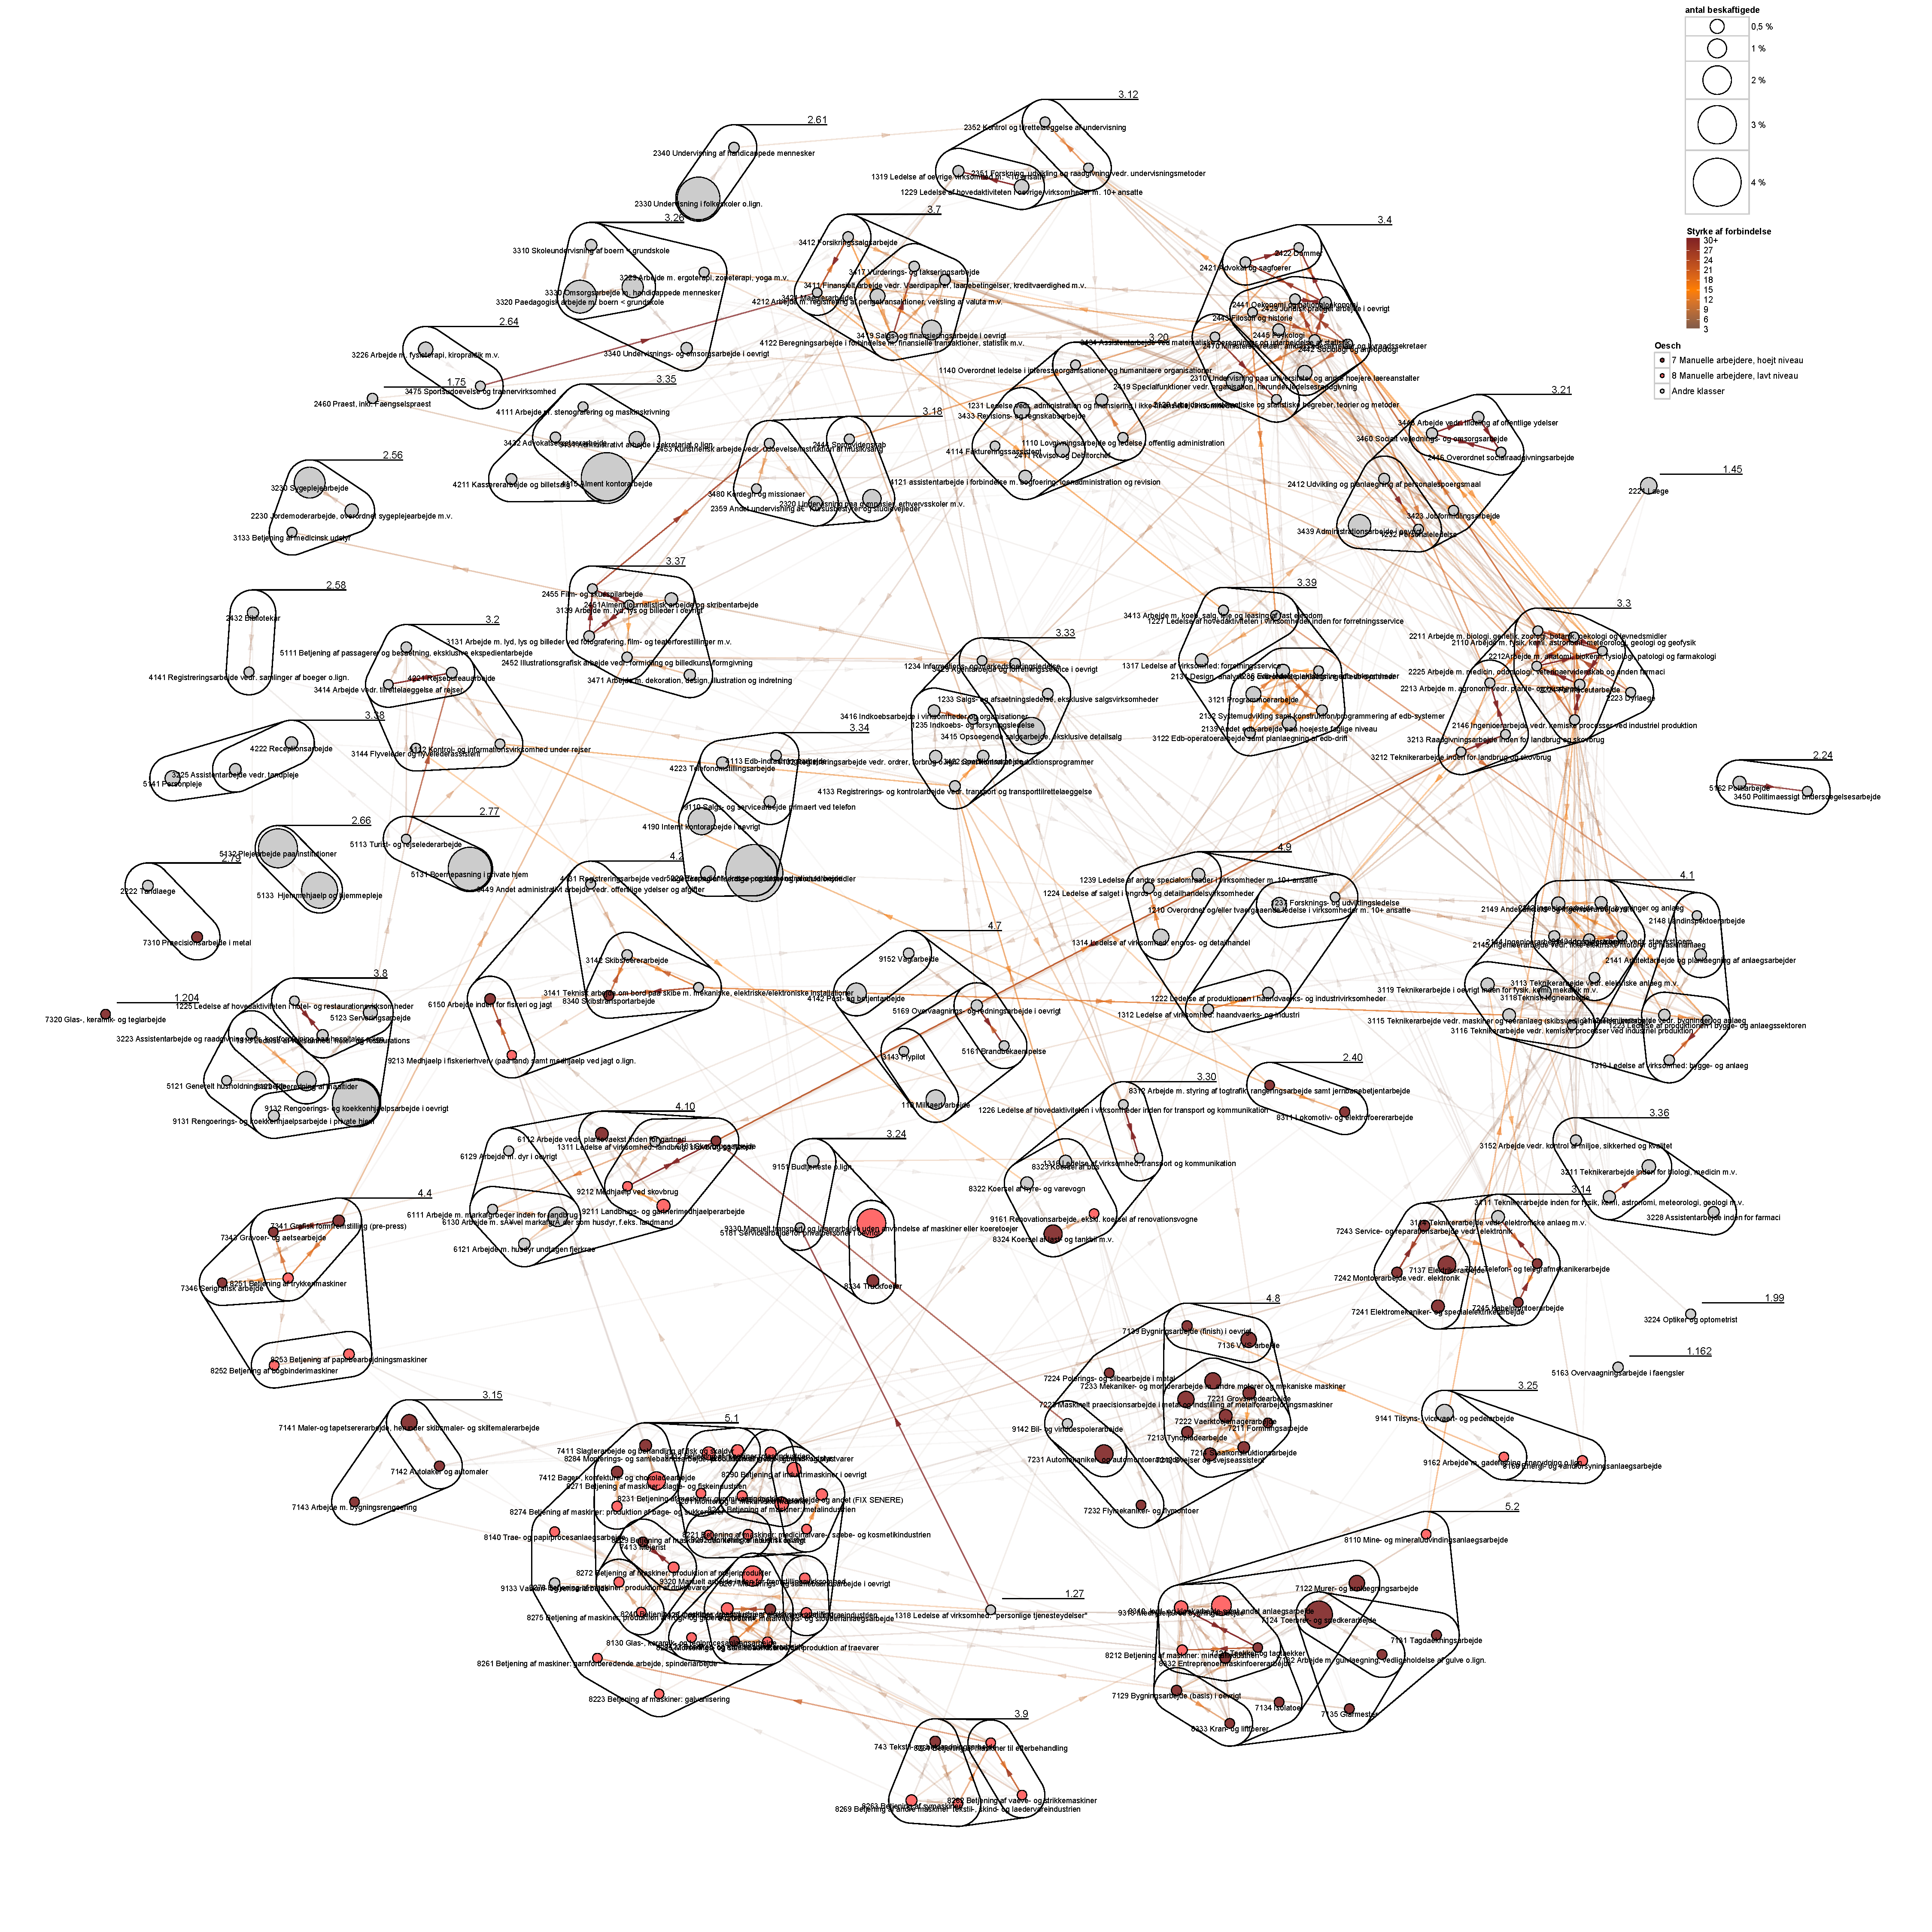
\includegraphics[width=\textwidth]{fig/netvaerkskort/kort_fokus_manuel_nonmanuel_roedgraa.pdf}
    \label{fig delanalyse3 klasse manuelt ikkemanuel}
   \end{centering}
   \end{figure}   
%


Langt de fleste af de erhvervsgrupper, der i Oeschs klasseskema er kategoriseret som manuelle arbejdere, er i samme segmenter. det ses også, at klassefraktionerne \emph{højere} og \emph{lavere} manuelt arbejde formår at at indfange de permabilitetsbarrierer, jeg tidligere har argumenteret for som centrale aspekter af hvad klasse er. Det er denne afhandlings unikke kombination af data på populationsniveau og en nyskabende netværksorienteret tilgang, der gør det muligt at undersøge dette aspekt af klasse. Det er derfor ganske spændende - og betryggende! at Oesch' klasseskema rent faktisk formår at ramme rimelig fornuftigt.

Der er imidlertidig undtagelser, der kan deles op i tre tendenser. De første to er generelle for de fleste klasser, mens den sidste er specifik for manuelle arbejderes mobilitet.

\underline{Den første tendens} omhandler de to, ganske vist manuelle, men højtspecialiserede erhvervsgrupper \emak{d7320} og \emak{d7310}. Disse to har en høj intern mobilitet på over 80 \%, og lader til at indfange en mesterlære-tradition, der fungerer effekt som social lukningsmekanisme. 

Dette kan forekomme som en underordnet pointe, men er alligevel en trend, der er ikke specifikt for den manuelle arbejderklasse, og derfor er værd at lægge mærke til, for at forstå mobilitet og faglige strategier generelt. Det ses indenfor de fleste klasser, eller, i en  \emph{teknicistisk} optik, indenfor hovedgrupperne i Disco-nomenklaturet: Enkelte erhvervsgrupper, - typisk erhvervsgrupper der kun indeholder \emph{en enkelt} profession - formår at fungerere som selvstændige delmarkeder. 
% Dette er ikke et centralt tema, men der er tydeligvis tale om en central del af arbejdsmarkedets struktur. 

Frank Parkin beskriver denne strategi som en strategi for at hæve egen markedsværdi, at erhvervet så at sige sørger for at have kontrol over egen arbejdskraft, og derved sikrer sig bedre vilkår og muligvis højere status end andre erhverv: “\emph{Professionalization itself may be understood as a strategy designed, amonst other things, to limit and control the supply of entrants to an occupation in order to safeguard or enhance its marked value}” \parencite[54]{Parkin1979}. Dette er ikke helt retvisende indenfor de to omtalte erhverv i den manuelle arbejderklasse, hvilket Parkin også skelner imellen. Professionelisering, e.g. adgangsgivende eksamener o.lign., er forskelligt alt efter om det sker som \emph{udbyttende} lukning, som indenfor højt bolige erhvervsgrupper såsom læger, eller om det er fagforeningsstrategier, hvis mål er at beskytte deres medlemmer mod udbytning. Forskellen er at det bevidste mål, i fagforeninger af den type Parkin mener, ikke har ævret at reducere de materielle muligheder for andre i arbejdsstyrken \parencite[57]{Parkin1979}. 
      % → det her skal stå et andet sted, i diskussionen, fx. For meget teori-tungt lige her. Bare kort i stedet, så det her ind et andet sted. 

\underline{Den anden tendens} handler om arbejdets genstandsfelt: \emph{Hvad} man arbejder \emph{med} er en betydningsfuld mekanisme i skabelsen af segmenter, og det ser ud til at komme an på genstandsfeltets relative størrelse i beskæftigelsesstrukturen, hvorvidt et sådan genstandsfelt dækker flere klasser eller ej%
%
    \footnote{ Ikke dermed sagt noget om deres størrelse i økonomien som sådan: Her spille landbruget en større rolle end dets relative andel af beskæftigede antyder. Det samme gælder skibsdrift, hvor Mærsk A/S næppe kan siges at være ubetydelig.}%
%
.  

Hvad jeg mener kan bedst illustreres med et eksempel. Segment \emak{s4.10} og segment \emak{s4.2} har begge en blandet  klassesammensætning, og her er det henholdsvis landbrug og skibsdrift, der er arbejdets genstandsfeltet. \emak{s4.10} indeholder 2,4 \% af arbejdsstyrken og \emak{s4.2} indeholder 0,5 \%. Disse segmenters arbejdsgenstandsfelt dækker en hel type af produktion, henholdsvis landbrug og skibsdrift. Fordi disse typer af produktion fylder så lidt i den overordnede samfundsmæssige produktion, er en lang række forskellige arbejdsfunktioner, på tværs af klasser, i samme segment. Det gør skift på tværs af klasse “\emph{let og typisk}”, hvilket ikke er tilfældet i genstandsfelter, hvor arbejdsdeling er langt mere specialiseret. 
Det ser vi tydeligt i de manuelle segmenter, hvis genstandsfelter rangererer fra fabriksarbejde i \emak{s5.1}, til håndværksklynger som \emak{5.2} og \emak{4.8} . De steder, hvor en stringent seriel opdeling af arbejdsprocesserne ikke mulig, ser ud til at være de steder, “\emph{hvor klasser mødes}”. Dette er netop et aspekt af arbejdskontrakten, som Goldthorpe lægger vægt på. %uddyb når du har styr på det

En anden, mere gængs måde at omtale forskellige typer af produktion på, kunne være \emph{sektorer i økonomien}. Det er tydeligt, at en sektor-baseret at en sektor-baseret tilgang også har en del at sige om mobiliteten på arbejdsmarkedet, og kunne være en nemmere måde end Moneca, hvorpå man kan  tage højde for de i realiteten segment-baserede opdelinger af arbejdsmarkedet. (vend tilbage til det her \#todo)


\underline{Den tredje tendens} er er de segmenter, hvor manuelle erhvervsgrupper befinder sig sammen med erhvervsgrupper fra andre klasser, typisk serviceklassens lavere fraktion. Dette er hvad man kunne klassens grænsetilfælde, og fungerer samtidig som de porte til andre typer af jobs, hvortil den manuelle klasse bevæger sig hen.  Det relaterer sig med en vis sandsynlighed til den omstrukturering af beskæftigelsesstrukturen, som jeg beskrev i afsnit \ref{henvisning til Oesch}.  De manuelle erhvervsgrupper, der her er i segment med andre klasser, er den manuelle klasses \emph{transporterhverv}, og findes i \emak{s3.24} og \emak{s3.30}, sammen med de ligeledes transport-relaterede erhvervsgrupper fra Oesch serviceklasse. For at fortælle denne historie, skal vi se på ændringen i antallet af beskæftigede indenfor segmenterne over tid i perioden, det vender jeg tilbage til i næste afsnit, på side \pageref{subsec delanalyse3 manuelle arbejdsklasse hvorhen mobilitet}.  %OG du skal se om det rent faktisk er sådan, at der er flere skift ud af den manuelle klasse end ind i den, som helhed og fra serviceklassen. undersøg det med R \#todo.

%
\subsection{Fordeling af beskæftigede i den manuelle klasses segmenter}
%



Så vidt undtagelserne. De fleste manuelle erhvervsgrupper befinder sig i samme segmenter. Alt i alt findes der 3 segmenter, der primært eller udelukkende består af lavt manuelt arbejde, 5 segmenter og én erhvervsgruppe, der primært eller udelukkende består af højt manuelt arbejde. Og 5 segmenter, hvori de manuelle jobs er blandet med andre klassekategorier, hovedsageligt fra serviceklassen. 

Segmenterne følger i det store og det hele Oesch distinktion mellem den højere og lavere fraktion af klassen. Et overblik over de forskellige segmenter, kategorieseret ud fra hvorvidt de består af at højere, lavere eller et blandet klassemiks, ses i tabel \ref{tab delanalyse3 fordeling manuel}.

    %!TEX root = ../report.tex
%
\begin{table}[H] \centering
\caption[Manuel klasse: Fordeling af beskæftigede i segmenter]{Fordeling af beskæftigede for den manuelle klasses segmenter}
\label{tab delanalyse3 fordeling manuel}
\resizebox{0.8\textwidth}{!}{%
% Table generated by Excel2LaTeX from sheet 'tab_manuelklasse_seg_miks'
% Table generated by Excel2LaTeX from sheet 'tab_manuelklasse_seg_miks'
\begin{tabular}{lrrrrrr}
Klasse & Andel beskæftigede & Kummulativ andel & Antal segmenter & Andel segmenter & Antal erhvervsgrupper & Andel erhvervsgrupper \\
\midrule
Manuelle arbejdere, højt niveau & 13\%  & 13\%  &                 6  & 13\%  &               41  & 15\% \\
Manuelle arbejdere, lavt niveau & 8\%   & 20\%  &                 3  & 6\%   &               39  & 14\% \\
Manuelle arbejdere, højt/lavt miks & 1\%   & 21\%  &                 1  & 2\%   &                 6  & 2\% \\
\midrule
Manuelle arbejdere og andre klasser & 8\%   & 28\%  &                 5  & 11\%  &               27  & 10\% \\
Andre klasser & 72\%  & 100\% &               32  & 68\%  &            160  & 59\% \\
\midrule
I alt & 100\% &       &               47  & 100\% &            273  & 100\% \\
\end{tabular} }
\end{table}
% 

 
Her ser vi hvorledes den manuelle del af arbejderklassen er delt op, hvis vores udgangspunkt er dens segmentering i delmarkeder og deres klasse. Den højere fagspecialisering, der findes i den manuelle klasses højere del, er en udmærket forklaring på, at denne klassefraktion består af flere segmenter end den lavere gør det. De indeholder omtrent samme antal erhvervsgrupper, men den lavere klassefraktion grupperer sig i halvt så mange segmenter som den højere. Det kan ikke forklares udelukkende ved at den højere manuelle fraktion beskæftiger 5 \% flere end den lavere manuelle fraktion. At erhvervsgrupperne grupperer sig sådan viser at det er nemmere at skifte job indenfor den lavere fraktion, hvilket ikke kun er en fordel: Det betyder også, at den enkelte person er nemmere at erstatte med en anden. 



Om de dele af arbejderklassen, der befinder sig i andre segmenter, bør inddrages, er et åbent spørgsmål. Mere om det senere, i første omgang vælger jeg at definere den manuelle klasse som bestående udelukkende af de segmenter, der består af klassens erhvervsgrupper. Dette mener jeg er formålstjenestligt, da de miksede segmenter, som jeg har været inde på, kan anskues på forskellig vis:

%
\begin{enumerate}
 \itemsep -0.5em
   \item Tilhører den manuelle klasse, men er indlejret i afgrænsede produktionsenheder, vis specialiserede genstandsfelt giver dem kompetencer, hvori integration med andre klasser er mulig  
   \item Erhvervsgrupper, der befinder sig i klassens grænseområde%
   %
       \footnote{ Som Bourdieu siger i \emph{Refleksiv sociologi: (find citat, det med klasser er som der hvor flammen stopper ved ilden \#todo )}}%
   %
   \item Tilhører ikke den manuelle klasse, dvs. forkert klassificeret i Oeschs skema
\end{enumerate}
%

Det vil jeg foreløbigt lade ligge, og arbejde videre med denne definition af den manuelle klasse: \emph{erhvervsgrupper der udelukkende befinder sig i segmenter med andre manuelle erhvervsgrupper.} Her bruger jeg Oeschs klassifikationsskema, som jeg kan konstatere har en udmærket overenstemmigelse med mine segmentdannelser, men modificeret ud fra den empiriske gruppedannelse, jeg kan observere. 

Klasse er, i det mindste for den manuelle klasses vedkommende, ikke en klasse “på papir”, som Bourdieu advarer imod teoretiske klassekonstruktioner. Det er vigtigt at påvise at en sådan har en realitet i handlingsmønstre, så det ikke kun udtrykker en \emph{sandsynlig} gruppering, men en \emph{faktisk observarbar} gruppering \parencite[7]{Bourdieu1987}. Det er netop, hvad jeg dermed har påvist i de menneskers jobmobilitetsmønstre, som har en fælles, fysisk manuel arbejdsform. Hvis du er i de manuelle segmenter, så er der en god mulighed for, at det er der, du bliver: Det er de mennesker, du omgås med 8 timer om dagen 5 dage om ugen de fleste ar årests måneder, og det er de lønninger, arbejdsforhold og pensionstyper, der findes indenfor den type arbejde, som former dine muligheder. Uden dermed sagt, at de deler \emph{andet} end dette, vil jeg alligevel mene, det er ret meget at dele. 


Jeg kan altså bekræftige samt justere Oesch klasseinddeling, hvilket jeg vil mene er et værdifuldt bidrag til at validere klasse som nyttig konstruktion. Men hvad betyder det så for arbejdsmarkedets funktionsmåde, og disse menneskers muligheder? 

Som jeg viste i afsnit \ref{fig teori tid Oesch8}, er tendensen i Danmark såvel som i andre vesteuropæiske lande, at andel af manuelt beskæftigede svinder ind, mens servicearbejdet stiger. Dette var imidlertidig ud fra Oeschs a priori klasseskema, der er designet til at dække alle moderne, vestlige lande. 



Jeg vil nu se på, hvordan mit udgangspunkt i mobilitetsmønstre kan bruges. Jeg vil mene, at et sådant udgangspunkt gør det muligt at se nærmere på hvilke trends, der er at spore i klasseudviklingen, og det er udviklingen i klassesammensætningen over tid, jeg nu vil gennemgå.

%
\subsubsection{En forfaldshistorie? \emph{- den manuelle klasses diminituering} (dumt ord find bedre \#todo)}
%
 

I kapitel \ref{kapitel_teori_klasse}, figur \ref{fig teori tid Oesch8} på side \pageref{fig teori tid Oesch8} påviste jeg, hvordan Danmark følger samme overordnede mønster i beskæftigelsesstrukturen som de andre vesteuropæiske lande, som Oesch undersøger: Den manuelle arbejderklasse skrumper, mens serviceklassen øges. Nu har jeg så påvist påvist, at Oesch klasseskema i meget høj, nærmest perfekt, grad lever op til denne afhandlings \emph{reason d'etre}, mobilitetsbarrierer på arbejdsmarkedet. Dermed er det trivielt at konstatere, at de segmenter, klassen består af, \emph{også} falder. Det er dog mindre trivielt, og i høj grad \emph{også} denne afhandlings reason d'etre, hvis jeg kan sige det uden at misbruge den vending, at de konkrete beskæftigelser, som klassen består af, ikke nødvendigvis følger samme trend. At se på segmenter som jeg gør her, kan netop, i modsætning til ren klasseteori, være med til at give konkret forståelse af de erhverv, folk rent faktisk lever deres liv i. På et policy-plan er det meget konkret anvendeligt, at forstå hvordan man kan håndtere de delmarkeder, hvori flaskehalsproblemer opstår. I figur \ref{fig delanalyse3 klasse tid manueltsegment} ser vi udviklingen i den manuelle arbejderklasses segmenter over tid. 

%
   \begin{figure}[H]
   \begin{centering}
    \caption[Tidsserie: De manuelle arbejdersegmenter]{De manuelle arbejdersegmenter, udvikling i andel beskæftigede i perioden 1994-2009. Segmenter med < 1 \% beskæftigede er summeret til én gruppe, af overskuelighedshensyn.} % du kunne lave en aggregeret gruppe med dem, og tegne dem som samlet gruppe. bare en ide, \#todo
    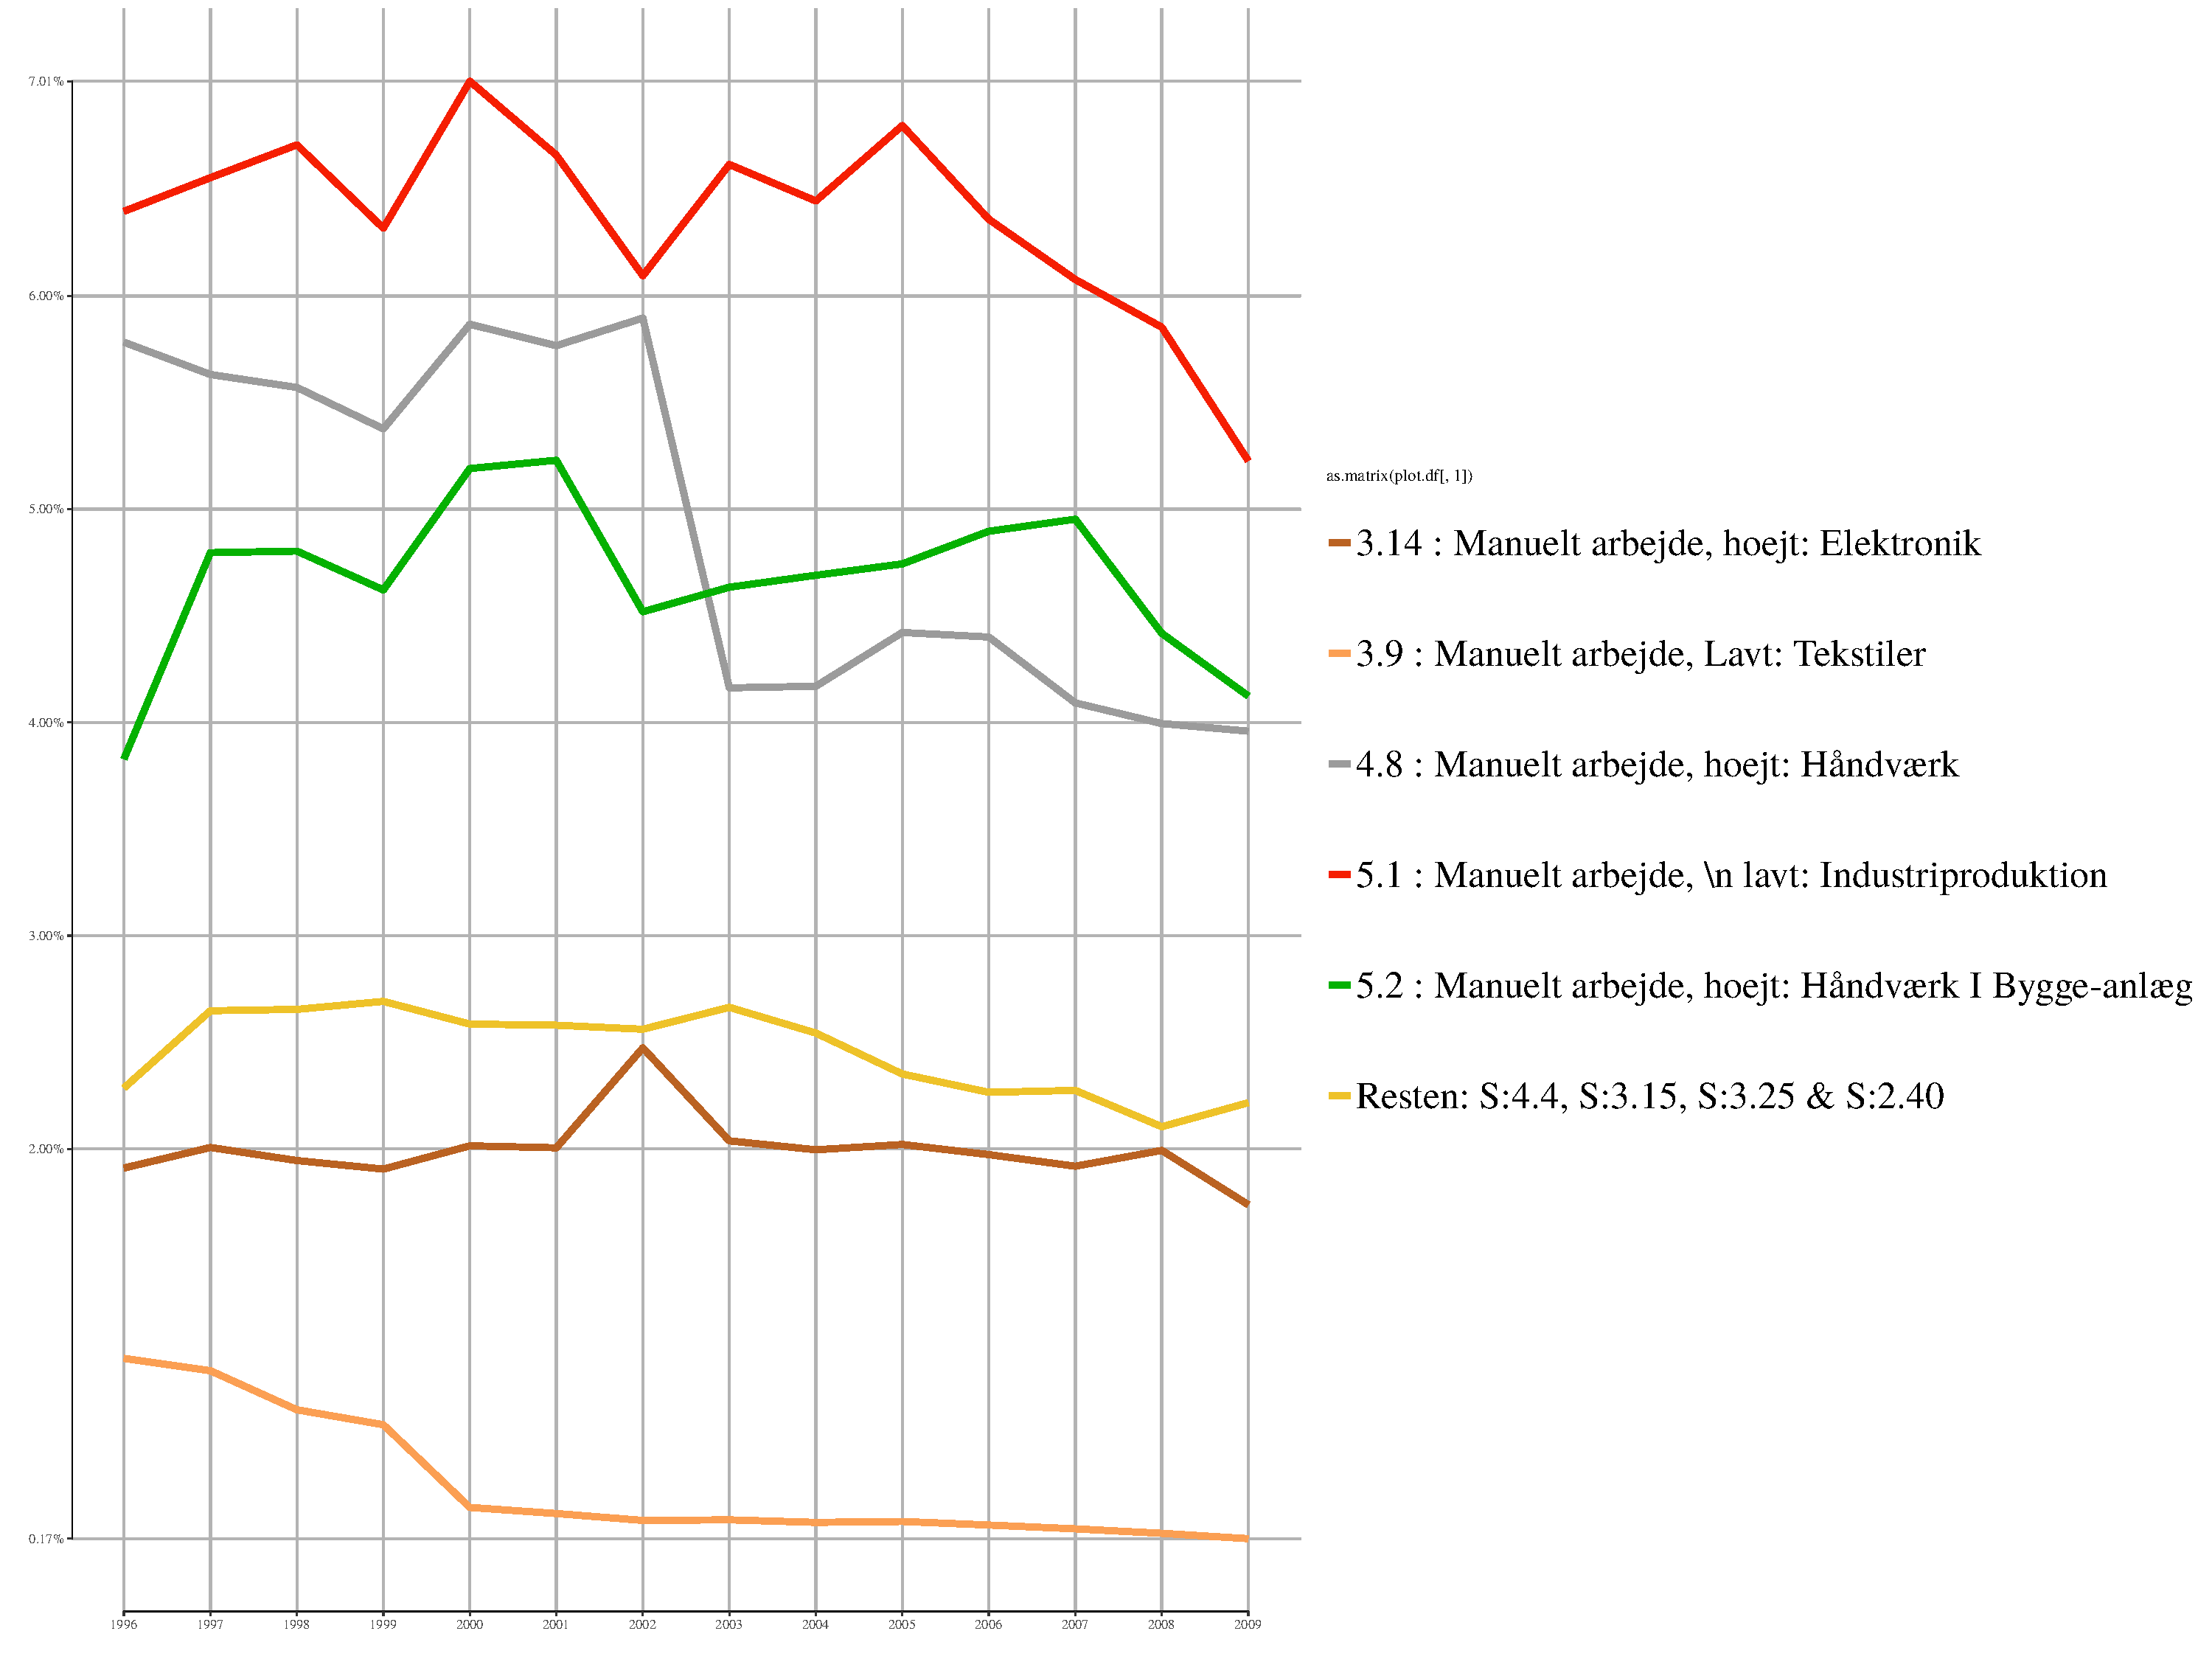
\includegraphics[width=\textwidth]{fig/tidsserier/tid_seg_manuelt.pdf}
    \label{fig delanalyse3 klasse tid manueltsegment}
   \end{centering}
   \end{figure}   
%

Vi lærer to ting ved at se på segmenterne. Det første er at det er 3 segmenter, der er drivkraften i tendensen til det støtte fald i manuelle jobs gennem midt-90'erne og 00'erne. To af dem ikke bare den manuelle klasses største segmenter, men \underline{hele} arbejdsmarkedets største segmenter, \emak{s5.1} og \emak{s4.8}.

I tabel \ref{tab delanalyse3 manuelklasse beskaeftigelse tid} ser vi forskellen fra 1996 til 2009, og det er en dramatisk udvikling: $\nicefrac{1}{5}$ af arbejdspladserne er forsvundet. Håndværkssegmentet og industriarbejderne er hårdt ramt. I procentvist fald er tekstilarbejderne nærmest forsvundet fra det danske produktionslandkort, omend det ser ud til, med figur \ref{fig delanalyse3 klasse tid manueltsegment} in mente, at det er en udvikling der starter et stykke tid før 1996, og ser ud til at nå sit lavpunkt omkring år 2000.




%
%!TEX root = ../report.tex
%
\begin{table}[H] \centering
\caption[Manuel klasse: Fald beskæftigelse i perioden 1996 til 2009]{Faldet i beskæftigelse for den manuelle klasse, fordelt på segmenter, arrangeret efter andel af alle beskæftigede}
\label{tab delanalyse3 manuelklasse beskaeftigelse tid}
\resizebox{0.8\textwidth}{!}{%
% Table generated by Excel2LaTeX from sheet 'tab_manuelklasse_tid'
\begin{tabular}{lrrrr}
Segment & \multicolumn{1}{l}{Beskæftigede 1996} & \multicolumn{1}{l}{Beskæftigede 2009} & \multicolumn{1}{l}{forskel} & \multicolumn{1}{l}{forskel i andel} \\
\midrule
4.8 : Manuelt arbejde, højt: Håndværk & 5,8\% & 4,0\% & -1,8\% & -31,5\% \\
5.1 : Manuelt arbejde,lavt: Industriproduktion & 6,4\% & 5,2\% & -1,2\% & -18,3\% \\
3.9 : Manuelt arbejde, Lavt: Tekstiler & 1,0\% & 0,2\% & -0,9\% & -83,4\% \\
3.14 : Manuelt arbejde, højt: Elektronik & 1,9\% & 1,7\% & -0,2\% & -8,9\% \\
Resten: S:4.4, S:3.15, S:3.25 \& S:2.40 & 2,3\% & 2,2\% & -0,1\% & -2,6\% \\
5.2 : Manuelt arbejde, højt: Håndværk I Bygge-anlæg & 3,8\% & 4,1\% & 0,3\% & 7,6\% \\
\midrule
I alt & 21,2\% & 17,4\% & -3,8\% & -21,7\% \\
\end{tabular} }
\end{table}
% 
% 
%


forklar tabellen her \#todo

Det er tydeligt, at det særligt det traditionelle fabriksarbejde i segment \emak{s5.1} og håndværkerfagene i segment \emak{s4.8} er faldet betragteligt i perioden. Bygge-anlægssektoren oplever en svag stigning i andelen af beskæftigede. Men taget i betragtning af, at vores slutår er 2009,  det første hele år efter finanskrisens start i 3. kvartal 2008, er det højest sandsynligt, at dette segment i en lignende opgørelse fra 2010 ville følge samme trend som de andre store manuelle klassesegmenter.  

Man kan diskutere, om dette segment egentligt hører til i den manuelle arbejderklasse. Dette vil jeg gemme til senere, men foreløbigt konstatere, der er noget om snakken, når vi taler om et tilbagetog for den traditionelle arbejderklasse. 

Dette speciale skal ikke afklare dette spørgsmål. Men selvom  østeuropæisk arbejdskraft måske-måske ikke er en vigtig faktor i faldet i antallet af jobs i segmentet. Så er den bekymring, disse lønmodtagere har haft om deres jobsikkerhed, ikke været ubegrundet.

Jeg tolker dette som et eksempel på, at en bestemt klasseposition giver visse erfaringer, der kan have en politisk effekt: Dette speciale ser ikke på årsagerne til denne udvikling: Uanset om det er reelt \emph{er} østeuropæisk arbejdskraft, muliggjort gennem EU, der spiller en en rolle her, eller om det er industriproduktionens udskibning til Kina, så er det vigtige her, i min optik, at dette er en genkendelig kobling, der kunne tyde på, at det måske ikke er irrationelt endda, at de lavtuddannede frygter globaliseringen, og ønsker sig tilbage til nationalstaten fra midten af det 20. århundrede. (okay måske lidt for hurtig på aftrækkeren, skal have mere tid? Måske i perspektivering istedet? \#todo)

På baggrund af de referede statikker og undersøgelser, mener jeg, at Moneca netop her viser at ved at se på mobilitetsklynger, som disse segmenter er udtryk for, ser vi, hvordan bestemte klassefraktioner har en fælles social oplevelse, indenfor deres type job, og dette gør dem, som vi kan se i undersøgelserne, mere tilbøjelige til at følge en bestemt klassehandlen, der ikke behøver være \emph{kollektiv refleksiv}. (forklar bedre eller slet \#todo) 



\begin{landscape}


%
\section{Hvor går den manuelle klasse hen? \label{sec delanalyse3 manuelle arbejdsklasse hvorhen mobilitet}}
%


% For at skabe bedre overblik over den sociale logik i disse mobilitetsmønstre, benytter jeg mig af et klassebaseret syn på arbejsmarkedets indretning. Jeg mener at et klassebaseret blik på arbejdsmarkedets forskellige positioner gør det nemmere at se, hvilke typer arbejde, der ligger socialt set nærmest for forskellige professioner, og det er mit formål at se, om jeg med dette blik er bedre i stand til at forklare disse mobilitetsmønstre.

% Samtidig oplever \emak{s3.24} og \emak{s3.30} stigninger. Segment \emak{s3.24} er den ene af de to transport-klynger med manuelle arbejdere, og her er genstandsfeltet transport \emph{ af varer}. \emak{s3.30} oplever en mindre, omend stadig stabil, stigning i beskæftigelsen, og har at gøre med kørsel, der i mindre grad er fokuseret på varetransport. I denne klynge er det interessant, at ledelses-klasserne indenfor genstandsfeltet bevæger sig i samme \emph{segmentet} som de klasser, hvis arbejde de leder og fordeler.  

Foruden selve etableringen af segmenter, er en netværksanalytisk metode som Moneca oplagt til at se på, er hvilke mobilitetskanaler, der så findes mellem arbejdsmarkedets segmenter.  først vil jeg... blah blah derefter vil jeg... blah blah og til sidst vil jeg... sove!




%
\subsection{Overblik over den manuelle klasses bevægelser \label{subsec_}}
%


I figur \ref{fig delanalyse3 manuelklassehoj without.mob disco} og \ref{fig delanalyse3 manuelklasselav without.mob disco} ses de ti erhvervsgrupper, hvor lønmodtagere fra henholdsvis den manuelle klasses højere og lavere fraktion hyppigst går til.

Lorem ipsum dolor sit amet, consectetur adipisicing elit, sed do eiusmod
tempor i


%
\subsubsection{Den højere manuelle klasses udadgående mobilitet}
%


Figur \ref{fig delanalyse3 manuelklassehoj without.mob disco} er et varmekort: En frekvenstabel eller krydstabel, hvor cellernes farve angiver deres værdi. For at enkelte meget høje værdier ikke skal forhindre aflæsningen af forskelle mellem de værdier, de fleste celler indeholder, er der sat en max-værdi for skalaen, som kan aflæses til højre. I selve cellen står dens præcise værdi. 

Dette varmekort viser andelen af mobilitet fra segmenter af den højere del af klassen til andre segmenter, inklusiv den lavere fraktion af samme. Hver celle er enten en erhvervsgruppe, et segment eller \emph{de resterende erhvervsgrupper i et segment}. 

Det skal forstås sådan, at tabellen er produceret, så alle erhvervsgrupper, der selvstændigt modtager over 750 skift fra klassefraktionen, får en selvstændig plads i tabellen. Derefter er de resterende erhversvgrupper summeret indenfor deres segment. Hvis et segment nu kan mønstre over 750 skift, får segmentet en plads i tabellen. Hvis det ikke kan, ender det i den sidste celle til venstre. Det betyder også, at hvis en enkelt erhvervsgruppe indenfor en eller flere erhversgrupper indenfor et segment selvstændigt indeholder over 750 skift, får de i en plads i tabellen, mens de resterende erhvervsgrupper i segmentet summeres. 

Tabellen er rangeret efter hvor stor en andel mobilitet, et segment modtager i alt fra klassefraktionen. Hvis et segment både indeholder erhvervsgrupper, der retfærdiggør en selvstændig plads i tabellen, og en summeret celle med resten af segmentet, er resten af segmentet placeret bagerst, så de selvstændige erhvervsgrupper fremhæves. 

Hvilke celler der hører til hvilket segmentet er fremhævet med et farvekodet panel og  en lille afstand.  

% erstat punktum med kommer med substr() eller gsub(), og tilføj en "total" bagved "Andre"-gruppen. lav desuden et objekt du kan kigge på med kummulative andele, og gerne så du kan se hele segmentet grupperet sammen også. tilføje måske hvor mange erhvervsgrupper i de resterende segmenter, hmm.  \#todo


\begin{figure}[H]
\begin{centering}
  \caption[Manuel klasse, højere: Mobilitet til erhvervsgrupper udenfor klassen]{Den udadgående mobilitet til erhvervsgrupper udenfor den manuelle klasses højere fraktion}
\label{fig delanalyse3 manuelklassehoj without.mob disco}
  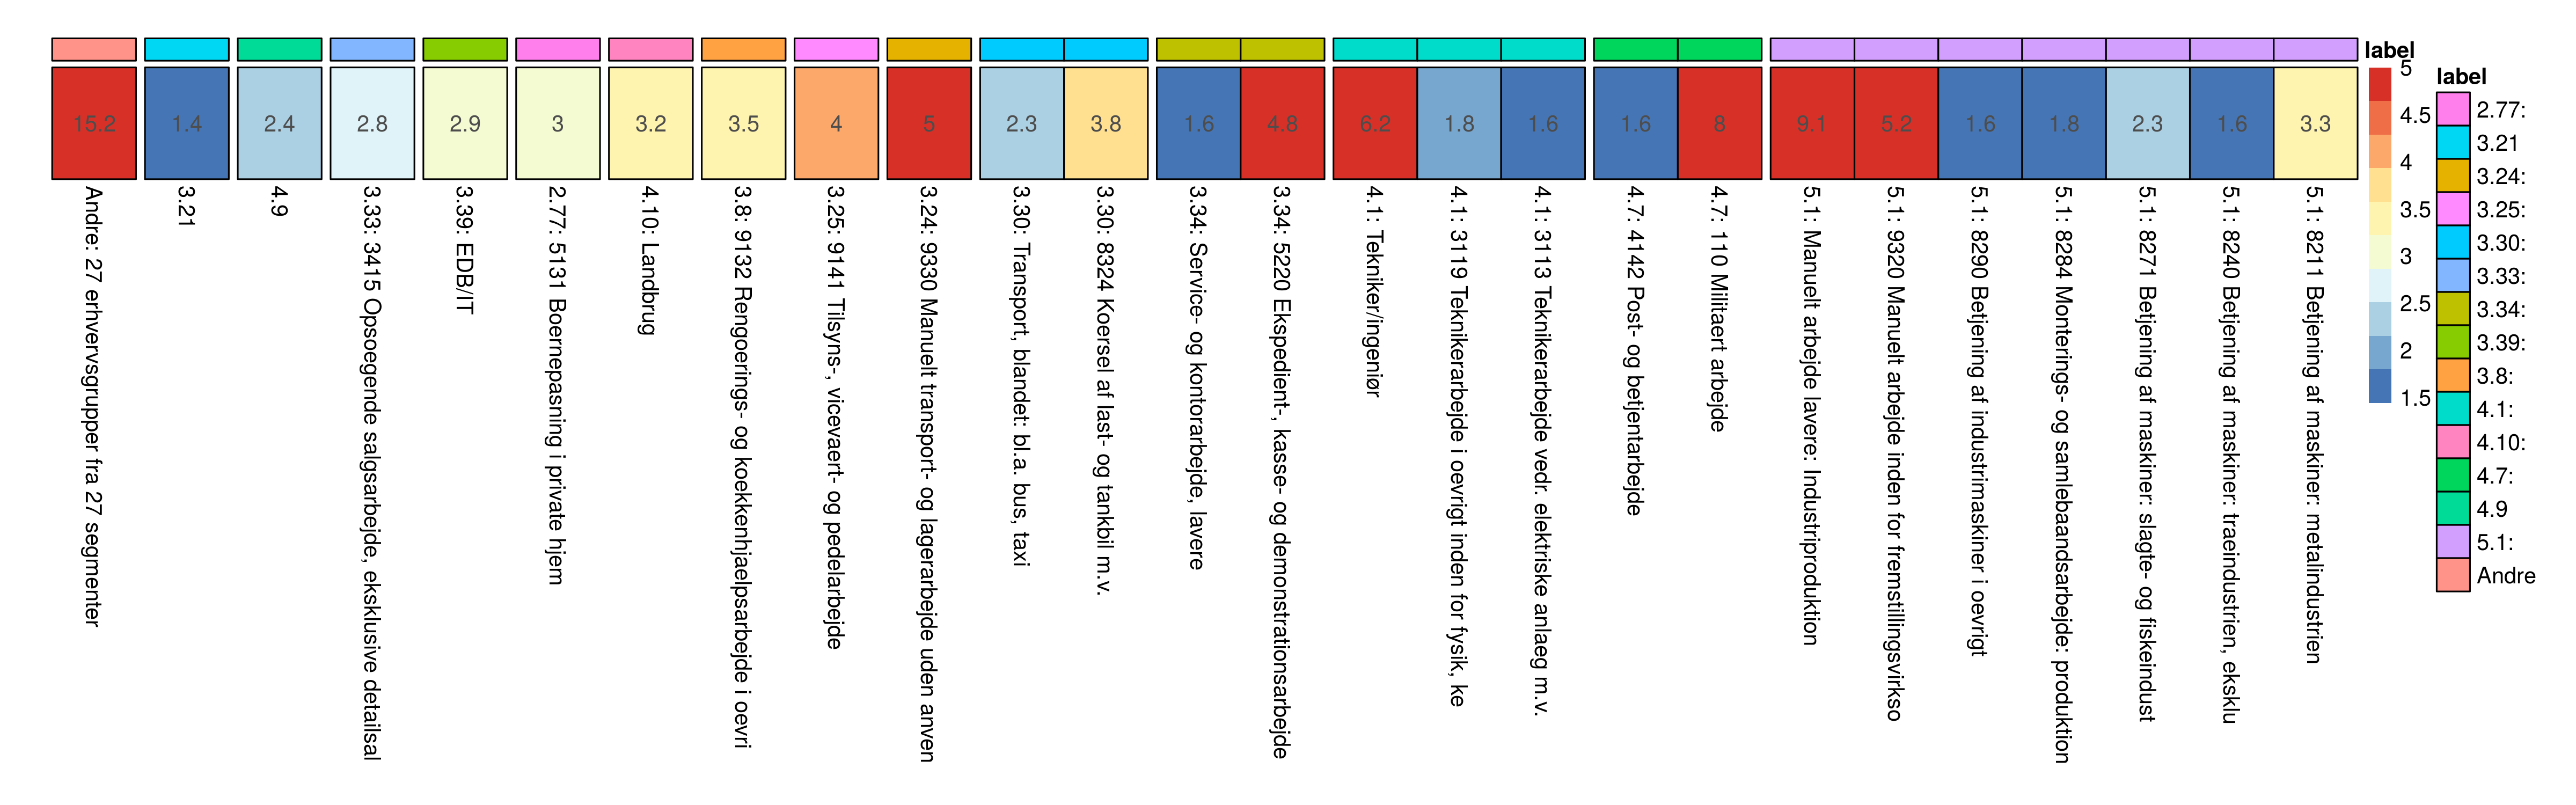
\includegraphics[width=\paperwidth]{fig/ma_motor/manuel_seg_hoj.png}
  % \label{fig delanalyse3 manuelklasse fokus}
\end{centering}
\end{figure}


Den største aftager af mobilitet fra den højere fraktion af den manuelle klasse, er den lavere fraktion af den manuelle klasse. Det er segmentet \emak{s5.1}, der opsamler fjerde jobskift (24,8 \%) fra den højere manuelle klasse. Der er ikke et særligt erhverv indenfor segmentet, der trækker denne tendens, hvilket er i god overenstemmigelse med det mønster, som det overordnede segmenteringskort viser, nemlig at de lavere manuelle erhverv er tæt forbundne, helt konkret gennem de mennesker, der udfylder dem.

I modsætning til denne generelle mobilitet over til industriproduktion, er næststørste arvtager kort og godt, militæret. Denne erhvervskategori er med 8 \% den største enkeltstående modtager af tidligere beskæftigede i højere manuelt arbejde. \emak{d110} er en del af et segment, hvis funktion i samfundet er sikkerhedsrelateret arbejde: vagt og betjentarbejde, og postuddeling %
%
    \footnote{ Det er en sær konstruktion i DISCO, at postarbejde er sat sammen med betjentarbejde, selv på det 4-cifrede niveau. Det er sandsynligt at en Moneca-analyse på et 6-cifret niveau havde splittet disse funktioner op i to, baseret på forskelle i deres mobilitetsmønstre. \emph{I guess we'll never find out, and it's a crying shame, too.}}%
%
    
Den 3. største aftager med 9,6 \% er, klassificeret efter uddannelsesniveau, et skridt op af: \emak{s4.1}. Det er værd at bemærke, da dette segment, sammen med de to ovenfor beskrevne, står for 45,2 \% af mobiliteten. Jeg vil senere vende tilbage til løn og ledighedstal indenfor disse segmenter, med henblik på at vurdere hvordan denne omstrukturering af beskæftigelsestrukturen medfører et økonomisk tab for de pågældende personer i manuelle og servicejobs.  \#todo

Den sidste ting dette varmekort fortæller os, er at segmenter, der er helt eller delvist domineret af servicearbejde, står for tilsammen 21,2 \% (tjek på præcise tal når du har vurderet alle segmenters klassekategori \#todo). 

I disse opgørelser skal man være opmærksom på, at der ikke kan skelnes mellem hvilke skift, der er udtryk for den manuelle klasses faldende andel af beskæftigelsen, altså en strukturel \emph{forskydning}, og hvilke, der skyldes en almindelig strukturel fluktation mellem forskellige klasser og klassefraktioner. 

Det er eksempelvis sandsynligt, at en del af denne mobilitet er sæsonbetinget, i forbindelse med arbejdsåret for eksempelvis tømrer og murer, hvor arbejdsmulighederne falder om vinteren, og mennesker i disse erhverv derfor søger andre jobs. Her ville et bud være, at en del af tilstrømningen til segment \emak{s5.1} skyldes denne type mobilitet, hvor mobiliteten så at sige vendes om, i en konstant bevægelse, ligesom ebbe og flod.

Den anden type mobilitet er den, der skyldes at hver 5. arbejdsplads er forsvundet i den højere manuelle klasses interne beskæftigelsesmuligheder \emph{(kig evt. på hele klassesegmenternes mobilitet og se, om der rent faktisk er sammenhæng her eller ej. \#todo). }. Om der er et sammenfald mellem at hver 5. job ud af det højere manuelle arbejde går til servicearbejde, kan jeg ikke udtale mig om med sikkerhed. Men et tentativt bud er, at denne mobilitet netop er udtryk for, om ikke alle, så en god portion af, de permanente skift.




% Det må betyde, at i gennemsnit hver 5. ikke vender tilbage til den manuelle klasses højere fraktion, men forbliver udenfor, eksempelvis i klassens lavere fraktion. Det er en gennemsnitsbetragtning, og det er sandsynligt at der er stor variation i, \emph{hvilke} segmenter, hvor de sæsonbetingede jobskift sker til, og de permanente skift. Man kan forestille sig, at flere sæsonbetingede skift sker til \emak{s5.1} end til \emak{s4.1}. Det ligger udenfor dette speciales rækkevidde at gå nærmere ind i dette, og jeg vil derfor holde mig til det bedste bud, som er gennemsnitsbetragtningen, og have dette forbehold i mente i den sikkerhed, hvormed jeg kan drage konklusioner om hvad man kunne kalde permanente og ikke-permanente skift.


% % 
% %!TEX root = ../report.tex
%
\begin{table}[H] \centering
\caption[Manuel klasse, højere: Mobilitet til erhvervsgrupper udenfor klassen]{Den udadgående mobilitet til erhvervsgrupper udenfor den manuelle klasses højere fraktion}
\label{tab delanalyse3 manuelklassehoj without.mob disco}
\resizebox{0.8\textwidth}{!}{%

% Table generated by Excel2LaTeX from sheet 'without_mob_manuel_hoj_disco'
\begin{tabular}{lrrr}
Erhversvgruppe & \multicolumn{1}{l}{Segment} & \multicolumn{1}{l}{Andel af mobilitet} & \multicolumn{1}{l}{Antal skift} \\
\midrule
110 Militaert arbejde & \multicolumn{1}{l}{4.7: Blandet, lavere: Vagt og sikkerhedsarbejde} & 8,0\% &             4.180  \\
9320 Manuelt arbejde inden for fremstillingsvirksomhed & \multicolumn{1}{l}{5.1: Manuelt arbejde lavere: Industriproduktion} & 5,2\% &             2.721  \\
9330 Manuelt transport- og lagerarbejde u. Køretøjer/maskiner & \multicolumn{1}{l}{3.24: Service- og manuelt:, blandet, lavere:: Varetransport} & 5,0\% &             2.585  \\
5220 Ekspedient-, kasse- og demonstrationsarbejde & \multicolumn{1}{l}{3.34: Service- og kontorarbejde, lavere} & 4,8\% &             2.483  \\
9141 Tilsyns-, vicevaert- og pedelarbejde & \multicolumn{1}{l}{3.25: Manuelt arbejde, lavere: Bygningsvedligehold, energi og vandanlægsarbejde } & 4,0\% &             2.073  \\
8324 Koersel af last- og tankbil m.v. & \multicolumn{1}{l}{3.30: Transport, blandet: bl.a. bus, taxi} & 3,8\% &             1.971  \\
9132 Rengoerings- og koekkenhjaelpsarbejde i oevrigt & \multicolumn{1}{l}{3.8: Service: restaurationsbranchen, primært lavere} & 3,5\% &             1.819  \\
8211 Betjening af maskiner: metalindustrien & \multicolumn{1}{l}{5.1: Manuelt arbejde lavere: Industriproduktion} & 3,3\% &             1.694  \\
5131 Boernepasning i private hjem & \multicolumn{1}{l}{2.77: Service, lavere: Børnepasning i private hjem og rejseleder} & 3,0\% &             1.550  \\
3415 Opsoegende salgsarbejde, eksklusive detailsalg & \multicolumn{1}{l}{3.33: Management: Salgsarbejde, blandet} & 2,8\% &             1.439  \\
Resterende erhvervsgrupper: & 158   & 56,8\% &           34.161  \\
\midrule
I alt & 168   & 100,0\% &           56.676  \\
\end{tabular} }
\end{table}
% 
%  % manuel klasse, høj
% % 

% når du skriver fraktion eller lavere manuelle klasse, så skriv et sted at det ikke er en stilingtagen til om man kan kalde den lavere del af den manuelle klasse for en klasse i sig selv, det skyldes sproglig flyd. \#todo

%
\subsubsection{Den lavere manuelle klasses udadgående mobilitet}
%


Figur \ref{fig delanalyse3 manuelklasselav without.mob disco} viser den udadgående mobilitet for den lavere del den manuelle klasse, som består af segment \emak{s5.1}, segment \emak{s3.25}, segment \emak{s3.9}

\begin{figure}[H]
\begin{centering}
\caption[Manuel klasse,lavere: Mobilitet til erhvervsgrupper og segmenter udenfor klassefraktionen]{Den udadgående mobilitet til erhvervsgrupper og segmenter udenfor den manuelle klasses lavere fraktion}
\label{fig delanalyse3 manuelklasselav without.mob disco}
  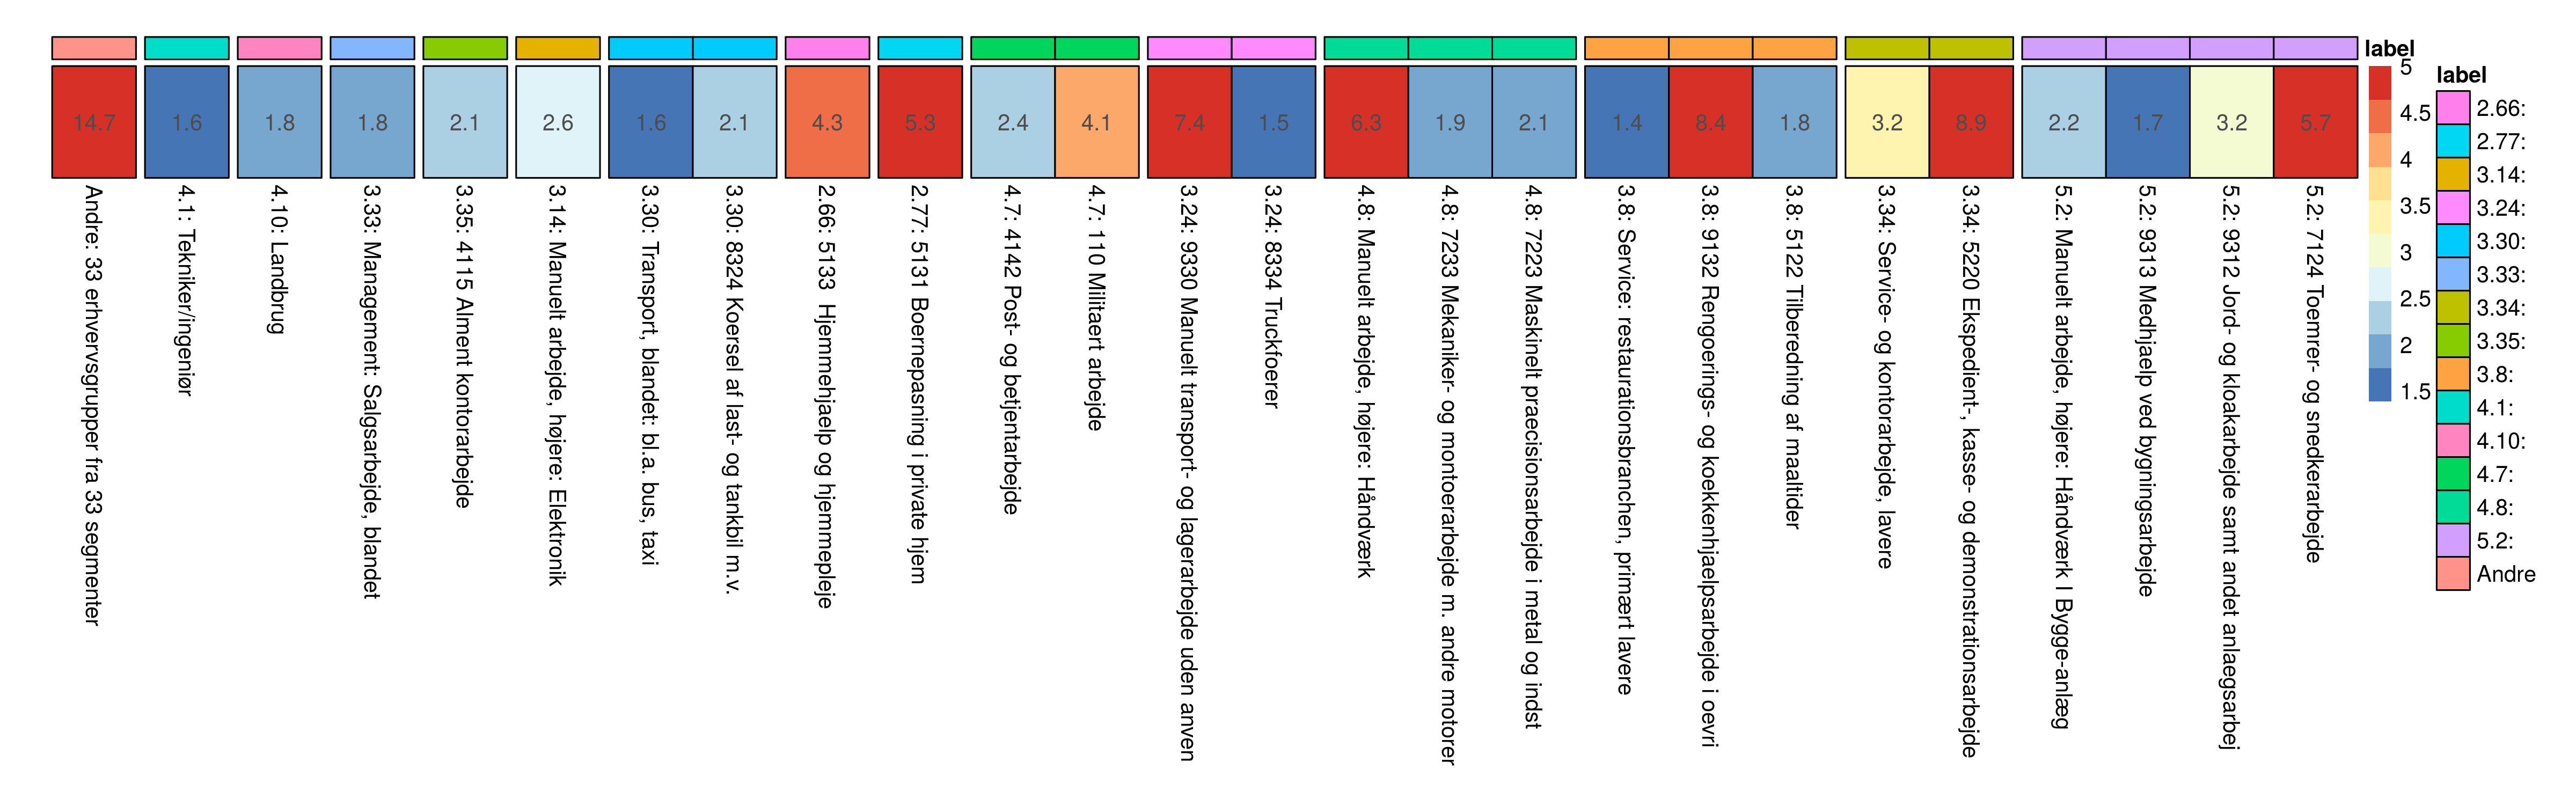
\includegraphics[width=\paperwidth]{fig/ma_motor/manuel_seg_lav.png}
  % \label{fig delanalyse3 manuelklasse fokus}% /sørg for at de tilsvarende tabeller med totaler kommer i bilag \#todo
\end{centering}
\end{figure}

I overenstemmigelse med min tese om, at “en hel del” af mobiliteten fra den højere manuelle klasse skyldes ikke-permanente skift, og er udtryk for et flux mellem de to klassefraktioner, ser vi, at også den lavere manuelle klassefraktion har stærke forbindelser til den højere ditto. 23.1 \% skifter til den højere manuelle klasse,  næsten præcis det samme antal som den modsate vej (24,8 \%). %tal ikke helt som de skal være endnu, vend tilbage \#todo
Da data er indsamlet over en 14 årig periode, og andelen begge veje er på ca. $\nicefrac{1}{4}$ for begge segmenter, konkluderer jeg, at det vi ser her er udtryk for en stabil struktur, altså ikke-permanente skift, grundet eksempelvis sæsonbetingede arbejdsvilkår. To af de fem segmenter, der hver især modtager ca. 10 \% af mobiliteten, er de to håndværkssegmenter i den højere manuelle klasse. Hvoraf ene er segment emak{s5.2}, altså det typiske sæsonbestemte arbejde.
%
    \footnote{ dette er en vurderingssag: Som nævnt før, kan der ikke foregå en tidsmæssig bestemmelse af hvornår på året, eller hvornår i \emph{årrækken}, at et jobskift er foregået. Det er derfor teoretisk muligt, at 24 \% af skiftene fra den lavere manuelle klasse til den højere foregik i 1996, og 0,8 \% skete i 2009. Mens det for den højere klasse var 0,1 \% der skiftede i 1996, og 23 \% der skiftede i 2009. Det kan ikke udelukkes, og jeg har  kke mulighed for at undersøge det i denne afhandling, ed den måde, data er struktureret på. %¤tdo  tag det med i perspektiveringen.
    Men i betragtning af den vægtige andel af det totale antal skift, der foregår begge veje, anser jeg det som meget sandsynligt, at der er tale om en stabil udveksling over årrækken, der ikke varierer voldsomt omkring gennemsnittet. På nuværende tidspunkt i monecas udvikling, er det heller ikke muligt at signifikansteste, det vil kræve en del nøje omtanke omkring de statistiske antagelser, hvis det ikke skal være rent symbolsk. Alligevel mener jeg, af de anførte grunde, at konklutionen er solid.}%
%
.  Hvis man lægger alle de højere manuelle segmenter sammen, er den samlede mobilitet fra den lavere manuelle klasse 29,5 \%.





% Begtrup:    Oesch8
% 8 Servicearbejdere  39.9  35.5
% 4 Manuelle arbejdere  38.7  40.1
% Begtrup:    Oesch16
% 15 Servicearbejdere, hoejt niveau   14
% 16 Servicearbejdere, lavt niveau    21.5
% 7 Manuelle arbejdere, hoejt niveau    25.5
% 8 Manuelle arbejdere, lavt niveau   14.6
% aabn_xls("./statistik/R/moneca/vores/voresdataframes/manuelle.klynger.lav.df.seg_beregninger_klasse.xlsx"

Så håndværksrelateret arbejde i den højere manuelle klasse er den ene store aftager fra den lavere manuelle klasse. Hvis vi ser på mobilitet til serviceklassen, er der en tydelig tendens at spore: Segmenter, hvis genstandsfelt primært er lavere serviceklassejobs, står for 52 \% af af mobiliteten, langt den største andel af den samlede mobilitet. Ud af disse 52 \% går 12,3 \% til den højere fraktion, og 39,7 \% går til den lavere fraktion%
%
    \footnote{ Husk at servicearbejdere, højere er kasse, ekspedient og demonstrationsarbejde. Det kunne man måske godt betvivle om det er rigtigt. \#todo}%
%

Der er, til forskel fra den højere fraktion af klassen, en meget tydelig systematik i hvilken mobilitet, der går til hvilke enkeltstående erhvervsgrupper. De tre største er \emak{d5220} (8,9 \%), \emak{d9132} (8,4 \%) samt \emak{d9330}%
%
    \footnote{ \emak{d9330} er godt nok klassificeret som manuelt arbejde af lavere grad i Oeschs skema, men hvis vi ser på hvor det \emph{relationelt} befinder sig, vil jeg mene det er at betragte som en serviceerhvervsgruppe, da det omhandler transport af goder, og befinder sig i segment sammen med servicearbejde, hvis genstandsfelt drejer sig om netop det.} 
    % argumenter eksempelvis for hvorfor det har ændret sig - det er \emph{blevet til} servicearbejde. \#todo
%
(7,4 \%). Det er kun ekspedientsarbejde, der er placeret på færdighedsniveau 2 på ISCEDs færdighedsskala, mens de to resterende, mere manuelt betonede erhvervsgrupper er klassificeret som færdighedsniveau 1. Det vil sige, at ekspedientarbejde kræver 2. halvdel af grundskolen færdiggjort, samt eventuelt en supplerende uddannelse, mens de to andre bare kræver 1. halvdel af grundskolen. Det er en klar indikator på, hvor tilgengængeligt arbejdet er for personer med lav eller ingen uddannelse.

Man kan med Goldthorpe og Parkins sige, at selvom dette arbejde er noget mindre klassificerbart end det fabriksarbejde, tidligere medlemmer af den lavere manuelle klasse kommer fra, så er det den form for servicearbejde, hvori arbejdskontrakten muliggør \emph{nem overvågning}, samt \emph{færdigheder, hvis erhvervelse ikke har nogen formelle sociale lukningsmekanismer}. Det gælder de fleste af de erhvervsgrupper, der modtager størstedelen af mobiliten fra den lavere manuelle klasse.

Der er enkelte undtagelser, såsom \emak{d2330}, hvortil 1,3 \% af mobiliteten går til, samt mobilitet til de to segmenter, der indeholder (de fleste fra) teknikker klasserne, tilsammen 3,6\%. 

Dete stiller et interessant spørgsmål: Hvor mange fra den manuelle klasse oplever et færdighedsløfti forbindelse med skift fra klassen? Der har været en smule tale blandt politikere om efteruddannelse, og fagforeninger har i mange år talt om nødvendigheden af det. Men når andelen af manuelt beskæftigede falder, er det så tale om et uddannelsesløft?

\end{landscape}

%
\subsubsection{Uddannelsesløft eller uddannelseskløft?}
%


For at svare på det spørgsmål, benytter jeg mig af ISCEDs hierarkiske klassifikation af arbejdsfærdigheder, som er en integreret del af DISCO nomenklaturet. Det er beskrevet på side ??? \#todo i kapitel \ref{kapitel_metode_datamateriale}. 

Nogle kommentarer omkring validiten af data bør nævnes, da jeg mener at konklutionerne jeg drager er solide: \underline{Det første} er at et skift fra den manuelle klasse til et højere færdighedsniveau ikke behøver være \emph{direkte} fra job til job: Min databehandling giver mulighed for mellemliggende perioder med uddannelsesforløb mellem jobskift. Eftersom den undersøgte periode spænder 14 år, kan datasættet godt opfange sådanne skift, selv med lange videregående uddannelsesforløb. \underline{Det andet er}, at  det er i starten af 00'erne, at det går nedad bakke for den manuelle klasse, og derfor burde en eventuel uddannelsesomstiling være med i data, hvis en sådan eksisterer. %vend tilbage til det her, se om det holder når du har opdateret ggplot2 tidsserierne for dine segmenter \#todo


Tabel \ref{tabel delanalyse3 withoutmob skillz} viser den udadgående mobilitet for den lavere manuelle klasse, fordelt på ISCED færdighedsniveauer. 


\begin{table}[htbp]
  \centering
  \caption[Manuel lavere klassefraktion: fordeling af mobilitet på ISCED færdighedsniveauer]{Fordeling af mobilitet på ISCED færdighedsniveauer i den lavere manuelle klasse.}
  \label{tabel delanalyse3 withoutmob skillz}%
  \resizebox{.8\textwidth}{!}{%
% Table generated by Excel2LaTeX from sheet 'without_mob_manuel_skill'
\begin{tabular}{lrrc}
ISCED færdighedsniveau & \multicolumn{1}{l}{udadgående mobilitet} & \multicolumn{1}{l}{andel udadgående mobilitet} & \multicolumn{1}{l}{kumulativ andel} \\
\midrule
1: Uden udddannelsesfærdigheder & 12851 & 23\%  & \multicolumn{1}{r}{23\%} \\
2: laveste færdighedsniveau (?KVU) & 34665 & 62\%  & \multicolumn{1}{r}{85\%} \\
3: mellemste færdighedsniveau (?MVU) & 4148  & 7\%   & \multicolumn{1}{r}{92\%} \\
4: højeste færdighedsniveau (?LVU) & 1378  & 2\%   & \multicolumn{1}{r}{94\%} \\
Heterogent færdighedsniveau & 851   & 2\%   & \multicolumn{1}{r}{96\%} \\
Militæret & 2288  & 4\%   & \multicolumn{1}{r}{100\%} \\
\midrule
I alt & 56181 & 100\% & - \\
    \end{tabular}}%
\end{table}%


Det ses, at langt den største del af mobiliteten går til færdighedsniveau 2 og 1, hvilket er 85 \% af mobiliteten, fordelt på 23 \% på færdighedsniveau 1 og 62 \% på færdighedsniveau 2. De resterende færdighedsniveauer står for 15 \%%
%
    \footnote{ Ingen af erhvervsgrupperne i den højere manuelle klasse befinder sig på et ISCED-færdighedsniveau > 2, så der behøves ikke tages forbehold for føromtalte ikke-permanente skift til denne klasse.}%
%
.  I selve lavere den manuelle klasse er andelen af jobs på færdigsniveau 1 på 27,1 \%, og færdighedsniveau 2 på 72,9 \%. Der er altså tale om en mindre forskydning til højere eller heterogene færdighedsniveauer, samt militæret, når de forlader klassen. Der er dermed i lav grad tale om, at individer fra den lavere manuelle klasse oplever et uddannelsesløft, når de bevæger sig ud af den manuelle klasse%
%
    \footnote{ Spørgsmålet er, hvor stor en andel af de mobilitetsskift, der foregår opad i færdighedsniveau, skyldes de faldende jobmuligheder i klassen, og hvor mange der skyldes en “naturlig”, mindre strøm af individer med ressourcer, der uanset konjukturerne har mulighed for at bevæge sig op af den sociale rangstige. Det vil sige, om de mennesker, der reelt ikke kan finde job, er en del af denne gruppe, der stiger i færdighedsniveau, eller om de blot bliver tvunget over i servicejobs. Det er et svært spørgsmål og besvare. Selvom denne tendes virker sandsynlig, og den ville betyde, at det lave uddannelsesløft reelt ikke skal tolkes som et løft, der har noget at gøre med forskydningen mellem klasserne, men blot en naturlig del af den sociale mobilitet, så er det ikke noget, jeg har mulighed for at undersøge her. Men det fortjener at blive nævnt.}%
%
. 

Tabel \ref{tabel delanalyse3 withoutmob skillz} viser samme fordeling af færdighedsniveauer for den højere manuelle klasse. 

\begin{table}[htbp]
  \centering
  \caption[Manuel højere klassefraktion: fordeling af mobilitet på ISCED færdighedsniveauer]{Fordeling af mobilitet på ISCED færdighedsniveauer i den højere manuelle klasse.}
  \label{tabel delanalyse3 withoutmob skillz}%
  \resizebox{.8\textwidth}{!}{%
% Table generated by Excel2LaTeX from sheet 'without_mob_manuel_skill'
\begin{tabular}{lrrc}
ISCED færdighedsniveau & \multicolumn{1}{l}{udadgående mobilitet} & \multicolumn{1}{l}{andel udadgående mobilitet} & \multicolumn{1}{l}{kumulativ andel} \\
\midrule
1: Uden udddannelsesfærdigheder & 10366 & 20\%  & \multicolumn{1}{r}{20\%} \\
2: laveste færdighedsniveau (?KVU) & 24419 & 47\%  & \multicolumn{1}{r}{67\%} \\
3: mellemste færdighedsniveau (?MVU) & 7867  & 15\%  & \multicolumn{1}{r}{82\%} \\
4: højeste færdighedsniveau (?LVU) & 3094  & 6\%   & \multicolumn{1}{r}{88\%} \\
Heterogent færdighedsniveau & 2064  & 4\%   & \multicolumn{1}{r}{92\%} \\
Militæret & 4180  & 8\%   & \multicolumn{1}{r}{100\%} \\
\midrule
I alt & 51990 & 100\% & - \\
    \end{tabular}}%
\end{table}%


Vi ser her en fordeling, der blah blah blah blah jeg gider ikke mere jeg er træt nu



2,8
84,6
12,5





\iffalse \label{iffalse}

http://www.dst.dk/da/Statistik/dokumentation/Nomenklaturer/DISCO-88/Introduktion.aspx%20


Uanset hvordan man vælger at klassificerer det, kan man tolke det, at gå fra eksempelvis tømrer til flyttemand er et trin ned af den sociale rangstige - dette vil blive tydeligere når vi ser på løn i delanalyse 2 (indsæt ref når du kommer til den \#todo). \emak{d9330} er en erhversvgruppe klassificeret som lavere manelt arbejde i Oesch klasseskema, men befinder sig i en klynge med servicearbejde. Hvis vi, som jeg vil argumentere for, betragter dette som et servicehverv, fordi omhandler \emph{transport af goder}, kan det tolkes som en omstillingsstrategi fra manuelle arbejdere fra en produktionsøkonomi til en serviceøkonomi. Det gælder også den 4. største erhvervsgruppe, der modtager tidligere lønmodtagere fra de højere manuelle segmenter: \emak{d5220}, der i sig selv er lavere servicearbejde, og tilhører et segment af lavere kontor- og servicearbejde.










Det ses af figur \ref{fig delanalyse3 manuelklasselav without.mob disco}, at de tre største enkeltstående erhvervsgrupper er \emak{d5220}, \emak{d9132} \emak{d9330}.











% (du bliver nødt til at finde ud af hvor meget mobilitet der går den modsatte vej for at kunne vurdere om det er en reel strukturændring eller bare en dynamik der ligger der. \#todo) % 8.9+8.4+7.4+5.3+4.3+2.1. 

 
%%!TEX root = ../report.tex
%
\begin{table}[H] \centering
% \caption[Manuel klasse: Fald beskæftigelse i perioden 1996 til 2009]{Faldet i beskæftigelse for den manuelle klasse, fordelt på segmenter}
% \label{tab delanalyse3 manuelklasse beskaeftigelse tid}
\resizebox{0.8\textwidth}{!}{%
% Table generated by Excel2LaTeX from sheet 'uadadgaaende_mob_manuel_disco'
\begin{tabular}{lrrr}
Erhversvgruppe & \multicolumn{1}{l}{Segment} & \multicolumn{1}{l}{Andel af mobilitet} & \multicolumn{1}{l}{Antal skift} \\
\midrule
5220 Ekspedient-, kasse- og demonstrationsarbejde & \multicolumn{1}{l}{3.34: Service- og kontorarbejde, lavere} & 9,7\% &           7.636  \\
9330 Manuelt transport- og lagerarbejde uden anvendelse af maskiner eller koeretoejer & \multicolumn{1}{l}{3.24: Service- og manuelt:, blandet, lavere:: Varetransport} & 8,8\% &           6.927  \\
9132 Rengoerings- og koekkenhjaelpsarbejde i oevrigt & \multicolumn{1}{l}{3.8: Service: restaurationsbranchen, primært lavere} & 8,4\% &           6.627  \\
110 Militaert arbejde & \multicolumn{1}{l}{4.7 Blandet, lavere: Vagt og sikkerhedsarbejde} & 8,3\% &           6.541  \\
5131 Boernepasning i private hjem & \multicolumn{1}{l}{2.77: Service, lavere: Børnepasning i private hjem og rejseleder} & 5,9\% &           4.667  \\
8324 Koersel af last- og tankbil m.v. & \multicolumn{1}{l}{3.30 Transport, blandet: bl.a. bus, taxi} & 4,1\% &           3.216  \\
5133  Hjemmehjaelp og hjemmepleje & \multicolumn{1}{l}{2.66 Service, lavere: Omsorgs- og plejearbejde} & 3,6\% &           2.856  \\
4142 Post- og betjentarbejde & \multicolumn{1}{l}{4.7: Blandet, lavere: Vagt og sikkerhedsarbejde} & 2,9\% &           2.255  \\
3415 Opsoegende salgsarbejde, eksklusive detailsalg & \multicolumn{1}{l}{3.33: Management: Salgsarbejde, blandet} & 2,7\% &           2.098  \\
4115 Alment kontorarbejde & \multicolumn{1}{l}{3.35: Management- og kontorarbejde, lavere} & 2,4\% &           1.913  \\
Resten, < 2 \%. antal erhvervsgrupper: & 139   & 43,3\% &        34.161  \\
\midrule
I alt & 149   & 100,0\% &        78.897  \\
\end{tabular} }
\end{table}
% 
%  % hele den manuelle klasse
% 







I tabel \ref{tab delanalyse3 without.mob manuel} ses de segmenter, som den største andel af mobiliteten fra de manuelle segmenter går til.  

%
%!TEX root = ../report.tex

%
\begin{table}[H] \centering
\caption[Manuel klasse: Udadgående mobilitet]{Udadgående mobilitet for den manuelle klasse, målt i antal og andel skift}
\label{tab delanalyse3 without.mob manuel}
\resizebox{0.8\textwidth}{!}{%
\begin{tabular}{lrrrr}
      & \multicolumn{1}{c}{Udadgående mobilitet, } &       & \multicolumn{1}{c}{Kummulativ} & \multicolumn{1}{c}{Andel af total} \\
\multicolumn{1}{c}{Segment} & \multicolumn{1}{c}{antal skift} & \multicolumn{1}{c}{Andel} & \multicolumn{1}{c}{andel} & \multicolumn{1}{c}{antal skift} \\
\midrule
3.34: Service- og kontorarbejde. lavt &           10.407  & 13\%  & 13\%  & 1,1\% \\
4.7: Vagt- og sikkerhedsarbejde &             9.779  & 12\%  & 26\%  & 1,0\% \\
3.8: Restaurationsbranchen &             8.960  & 11\%  & 37\%  & 1,0\% \\
3.24: Varetransport &             8.678  & 11\%  & 48\%  & 0,9\% \\
4.1: Tekniker og ingeniørarbejde &             6.047  & 8\%   & 56\%  & 0,6\% \\
3.30 Vare- og persontransport &             5.348  & 7\%   & 62\%  & 0,6\% \\
2.77: Privat børnepasning og rejseleder &             4.688  & 6\%   & 68\%  & 0,5\% \\
2.66: Omsorgs- og plejearbejde &             3.863  & 5\%   & 73\%  & 0,4\% \\
Andre segmenter &           21.127  & 27\%  & 100\% & 2,2\% \\
\midrule
I alt &           78.897  & 100\% & 100\% & 8,5\% \\
\end{tabular}}
\end{table}
% 
%
\emph{dit tal for absolut mobilitet er misvisende, fordi du ikke har sat mobilitet internt i segmenter til 0. Og det er jo det niveau, vi opererer på. Så gør det, eller fjern den kolonne. \#todo.}

I alt bevæger personer der er beskæftiget i den manuelle klasse sig til 35 segmenter, når de bevæger sig ud af den manuelle klasse. hvoraf det største antal skift til et segment er på 10.407 skift, mens det mindste er på 6 skift%
%
    \footnote{ ikke med i tabellen, men der er tale om den ikke-segmenterede, universitetsuddannelse \emak{d2221}.}%
%
. 

Mobiliten er koncentreret om 4 segmenter: segment 3.34, 4.7, 3.8 og 3.24. Disse udgør 48 \% af den samlede mobilitet. Det er segmenter, hvoraf en stor del af erhvervsgrupperne er fra serviceklassens nedre del. Jeg kan derfor konstatere, at væksten i antallet af servicearbejdere skyldes -  delvist ihvertfald - en omstrukturering af de mulige beskæftigelsesmuligheder for lavtuddannede. Dette har, naturligt nok, kunne man sige, den konsekvens, at manuelle arbejdere søger beskæftigelse i servicesektoren. Den voksende klasse af servicearbejdere består altså i nogen grad af tidligere arbejdere fra de manuelle erhverv (hvad er de sociale konsekvenser af det? kom nu hjerne, virk \#todo)

Den største kategori i tabellen “andre segmenter” samler 27 segmenter, hvor mobiliten fra den manuelle klynger hver for sig er under 5 \%, de fleste langt mindre. 


Det segment, der i figur \ref{tab delanalyse3 without.mob manuel} er en overraskende modtager af tidligere manuelle arbejdere, er segment \emak{s4.1}. Hvis man mener, og det gør de fleste jo, at social mobilitet er en værdi i sig selv, er det positivt, at manuelle arbejdere omskoler sig til mere (om ikke andet i uddannelsesmæssig og/eller symbolsk forstand) krævende arbejdsfunktioner.


Jeg kan hermed konstatere, at både den manuelle klasses lavere og højere fraktion bevæger sig til serviceklassens lavere del. I den højere fraktion af den manuelle klasse er der også en substantiel bevægelse til det lavere segment af samme klasse, men også her fylder bevægelsen mod serviceklassen det meste. Det og så arbejde i militæret, der ligger indenfor \emak{s4.7}, som man kan argumentere for er en indgang til sikkerhedsbaserede servicehverv som vagt. hvilken klasse er det. \#todo







%
\subsection{kort over den manuelle klasses bevægelser}
%

Til det fokuserer jeg Moneca-kortet på de bevægelser, der går fra de manuelle arbejderes segmenter. Det er afbilledet i figur \ref{fig delanalyse3 manuelklasse fokus}.

Den vigtige forskel fra tidligere kort, er at forbindelserne på kortet ikke viser den (relative) måleenhed relativ risiko. Forbindelserne her viser det reelle antal skift. Dette skyldes, at hvor det i Monecas klyngedannelsesproces og generelle netværksstruktur er hensigtsmæssigt at vise forbindelser \emph{relativt} til erhvervsgruppernes størrelse, som redegjort for i afsnit \ref{metode_relativrisiko}, er vi her interesseret i at se på det faktiske antal jobskift. 



 Den anden forskel er at kortet kun viser forbindelser \underline{fra} erhvervskategorier inden for den manuelle klasse, \underline{til} erhvervskategorier udenfor klassen%
%
    \footnote{ Det vil sige bevægelse mellem de manuelle segmenter også er udeladt.}%
%
. 

Endelig skal nævnes farvelægningen af erhvervsgrupperne. Disse er farvelagt efter klassesammensætningen af det segment de befinder sig i, ud fra min opdeling i tabel \ref{tab delanalyse3 fordeling manuel}:
De manuelle klassesegmenter er mørkerøde. Den lave del af den manuelle klasse er lys rød, mens segmentet med et miks af de to fraktioner er mellemrød. De 4 segmenter hvori manuelle erhvervsgrupper indgår sammen med andre segmenter er orange. Alle andre segmenter end de segmenter, der indeholder manuelle erhvervsgrupper, er grå. Så det er kun forbindelser \underline{fra} de tre nuancer af rød \underline{til} orange eller grå klynger, der er afbilledet i kortet.

\begin{figure}[H]
\begin{centering}
  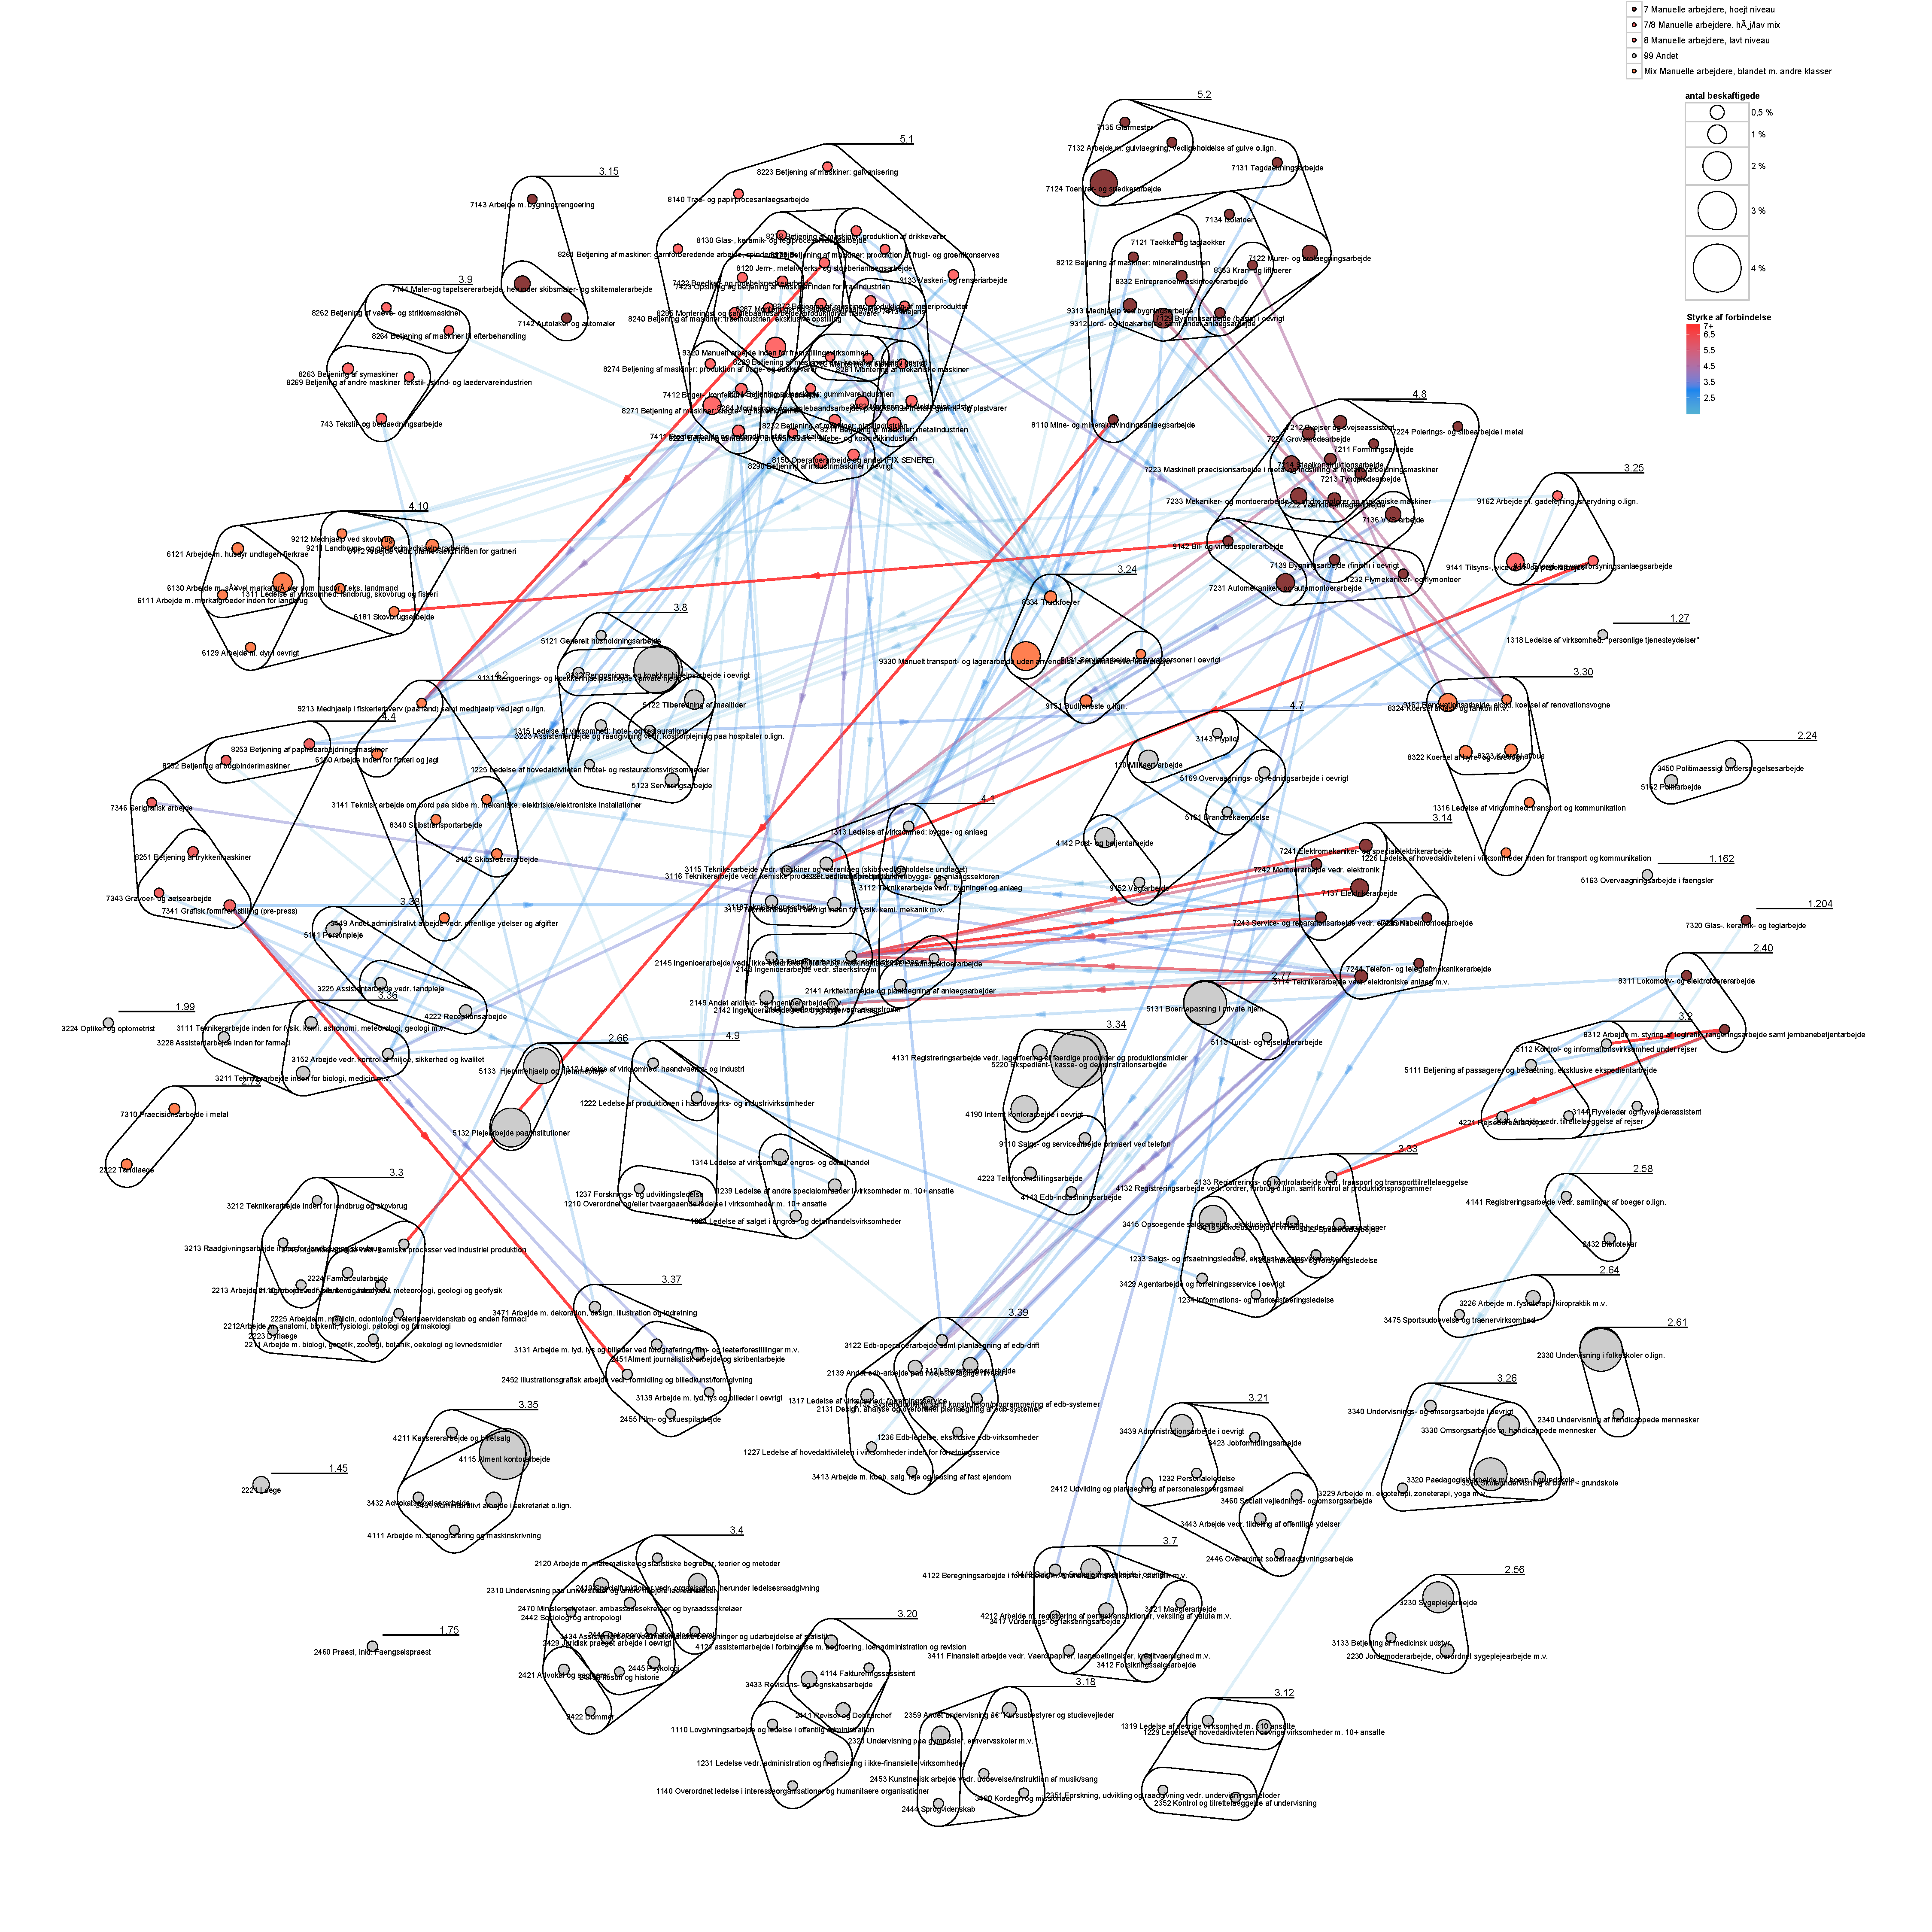
\includegraphics[width=10 cm]{fig/netvaerkskort/fokus_manuel_nonmanuel.pdf}
  \caption[Netværkskort: mobilitet fra den manuelle klasse]{Kort over de manuelle klasse-segmenters mobilitet til andre segmenter}
  \label{fig delanalyse3 manuelklasse fokus}
\end{centering}
\end{figure}




En række tendenser kan spores ud fra kortet. Det første er at segment \emak{s5.1}, der, som vi husker fra figur \ref{fig delanalyse3 klasse tid manueltsegment}, står for xx procent af faldet 


En betragtelig del af mobiliten til \emak{s3.34} kommer fra  går fra \emak{s5.1}. 












%%%%%%%%%%%%%%%%%%%%%%%%%%%%%%%%%%%%%%%%%%%%%%
% #Noter 
%%%%%%%%%%%%%%%%%%%%%%%%%%%%%%%%%%%%%%%%%%%%%%
% 
% 
%
%

% En sidste overordnet betragtning om det kønnede arbejdsmarked, er at det ser ud til, at den kvindelige fabriksarbejder - altså kvinder beskæftiget indenfor manufaktur fremfor service - ser ud til at være forsvundet fra arbejdsmarkedet % brug kun denne reference hvis du kan finde en reference på hvor mange kvinder der arbejdede som fabriksarbejder i kapitalismens guldalder \#todo

% http://www.leksikon.org/art.php?n=1504
% og læs Marianne Rostgaards artikel om kvindelige og mandlige arbejdere op gennem det 20. århundrede.









%%%%%%%%%%%%%%%%%%%%%%%%%%%%%%%%%%%%%%%%%%%%%%%%%%%%%%%%%%%

policy-ide:
Man kunne: spore skiftene via registerdata, og lave sociale profiler på *hvem* der skifter *hvorhen*, så man bedst kan vurdere, om det er smart








% %
% \begin{quote} \small %\raggedright %(bloktekst on/off)
% even if I was some twat who had a wife and a dog and a car that I took out for walks everyother fuckin' day, it's still fucking absurd to be describing anything this big, like, a monkey trying to grasp the structure of all other monkeys, \emph{including itself}, right? 
% \sourceatright{- Mig selv, d. 09//03//2017}
% \end{quote}
% %


% % 
% %!TEX root = ../report.tex
%
\begin{table}[H] \centering
\caption[Manuel klasse,lavere: Mobilitet til erhvervsgrupper udenfor klassen]{Den udadgående mobilitet til erhvervsgrupper udenfor den manuelle klasses lavere fraktion}
\label{tab delanalyse3 manuelklasselav without.mob disco}
\resizebox{0.8\textwidth}{!}{%

% Table generated by Excel2LaTeX from sheet 'without_mob_manuel_lav_disco'
\begin{tabular}{lrrr}
Erhversvgruppe & \multicolumn{1}{l}{Segment} & \multicolumn{1}{l}{Andel af mobilitet} & \multicolumn{1}{l}{Antal skift} \\
\midrule
5220 Ekspedient-, kasse- og demonstrationsarbejde & \multicolumn{1}{l}{3.34: Service- og kontorarbejde, lavere} & 8,9\% &              5.020  \\
9132 Rengoerings- og koekkenhjaelpsarbejde i oevrigt & \multicolumn{1}{l}{3.8: Service: restaurationsbranchen, primært lavere} & 8,4\% &              4.693  \\
9330 Manuelt transport- og lagerarbejde uden anvendelse af maskiner eller koeretoejer & \multicolumn{1}{l}{3.24: Service- og manuelt:, blandet, lavere:: Varetransport} & 7,4\% &              4.178  \\
7124 Toemrer- og snedkerarbejde & \multicolumn{1}{l}{5.2: Manuelt arbejde, højere: Håndværk I Bygge-anlæg} & 5,7\% &              3.179  \\
5131 Boernepasning i private hjem & \multicolumn{1}{l}{2.77: Service, lavere: Børnepasning i private hjem og rejseleder} & 5,3\% &              3.000  \\
5133  Hjemmehjaelp og hjemmepleje & \multicolumn{1}{l}{2.66: Service, lavere: Omsorgs- og plejearbejde} & 4,3\% &              2.410  \\
110 Militaert arbejde & \multicolumn{1}{l}{4.7: Blandet, lavere: Vagt og sikkerhedsarbejde} & 4,1\% &              2.288  \\
9312 Jord- og kloakarbejde samt andet anlaegsarbejde & \multicolumn{1}{l}{5.2: Manuelt arbejde, højere: Håndværk I Bygge-anlæg} & 3,2\% &              1.786  \\
4142 Post- og betjentarbejde & \multicolumn{1}{l}{4.7: Blandet, lavere: Vagt og sikkerhedsarbejde} & 2,4\% &              1.350  \\
8324 Koersel af last- og tankbil m.v. & \multicolumn{1}{l}{3.30: Transport, blandet: bl.a. bus, taxi} & 2,1\% &              1.207  \\
Resterende erhvervsgrupper: & 161   & 48,2\% &           34.161  \\
\midrule
I alt & 171   & 100,0\% &           63.272  \\
\end{tabular} }
\end{table}
% 
%  % manuel klasse, høj
% % 




% Dette sigte har et dobbeltrettet formål: Man kan sige, at den empiriske ramme, med dets unikke fokus på mobilitet forstået ud fra netværksmetode, skal lære os at forstå noget om hvad klasse \emph{er} i dagens Danmark. Og Oeschs moderne klasseteori er et teoretisk blik, der tillader os at begribe den komplekse klassestruktur, empirien viser os. 

% Mobilitet, særligt indenfor segmenterne, fortæller os, hvorvidt de teoretiske klasser, vi arbejder med, afspejler en social virkelighed, hvor mobilitet er “let og typisk”, som Weber sagde det. Så vurderingen går altså begge veje - fra klasse som måde at forstå mobilitetsmønstre på, og mobilitetsmønstre som en måde at forstå klasse på. 






% Trash 

%%%%%%%%%%%%%%%%%%%%%%%%%%%%%%%%%%%%%%%%%%%%%%%%%%%%%%%%%%%








\fi


